%%__________________________________________________________________||

%%__________________________________________________________________||
\RCS$Revision: 326816 $
\RCS$HeadURL: svn+ssh://svn.cern.ch/reps/tdr2/papers/SUS-15-005/trunk/SUS-15-005.tex $
\RCS$Id: SUS-15-005.tex 326816 2016-02-19 20:36:18Z sakuma $

%%__________________________________________________________________||
\cmsNoteHeader{SUS-15-005}

%%__________________________________________________________________||
\title{Search for new physics in final states with jets and missing
transverse momentum in $\sqrt{s}$ = 13 TeV pp collisions with the
$\alpha_{\text{T}}$ variable}

%%__________________________________________________________________||
\address[cern]{CERN}
\author[cern]{The CMS Collaboration}

%%__________________________________________________________________||
\date{\today}

%%__________________________________________________________________||
\abstract{An inclusive search for supersymmetric processes that produce final states with jets and missing transverse momentum is performed in pp collisions at a centre-of-mass energy of 13 TeV. A dimensionless kinematic variable, $\alpha_{\text{T}}$, is used to discriminate between events with genuine and misreconstructed missing transverse momentum. A data sample corresponding to an integrated luminosity of $2.2~\text{fb}^{-1}$, recorded by the CMS experiment at the LHC, is analysed. The observed signal candidate event counts are found to be in agreement with the expected contributions from standard model processes and the result is interpreted in the mass parameter space of supersymmetric simplified models.}

% 1. **DO NOT use \include or \input** to include the abstract: our
%    abstract extractor will not search through other files than this
%    one.
% 2. **DO NOT use %** to comment out sections of the abstract: the
%    extractor will still grab those lines (and they won't be
%    comments any longer!).
% 3. For PASs: **DO NOT use tex macros** in the abstract: CDS MathJax
%    processor used on the abstract doesn't understand them _and_ will
%    only look within $$. The abstracts for papers are hand formatted
%    so macros are okay.


%%__________________________________________________________________||
\newcommand{\kfactor}{\ensuremath{k\text{-factor}}\xspace}
\newcommand{\kfactors}{\ensuremath{k\text{-factors}}\xspace}
\newcommand{\njet}{\ensuremath{n_{\text{jet}}}\xspace}
\newcommand{\njetlow}{\ensuremath{2 \leq \njet \leq 3}\xspace}
\newcommand{\njethigh}{\ensuremath{\njet \geq 4}\xspace}
\newcommand{\nb}{\ensuremath{n_{\text{b}}}\xspace}
\newcommand{\alphat}{\ensuremath{\alpha_{\text{T}}}\xspace}
\newcommand{\alphatcut}{\ensuremath{\alpha_{\text{T}}^{\text{cut}}}\xspace}
\newcommand{\htalphat}{\texttt{HT\_AlphaT}\xspace}
\newcommand{\photon}{\texttt{Photon}\xspace}
\newcommand{\muht}{\texttt{Mu\_HT}\xspace}
\newcommand{\httrigger}{\texttt{HT}\xspace}
\newcommand{\mt}{\ensuremath{M_{\textrm T}}\xspace}
\newcommand{\gj}{\ensuremath{\gamma} + jets\xspace}
\newcommand{\mj}{\ensuremath{\mu} + jets\xspace}
\newcommand{\mmj}{\ensuremath{\mu\mu} + jets\xspace}
\newcommand{\npre}{\ensuremath{N_{\textrm{pred}}}\xspace}
\newcommand{\nobs}{\ensuremath{N_{\textrm{obs}}}\xspace}
\newcommand{\njets}{\ensuremath{N_{\textrm{jet}}}\xspace}
\newcommand{\sq}{\ensuremath{\tilde{\rm q}}\xspace}
\newcommand{\st}{\ensuremath{\tilde{\rm t}}\xspace}
\newcommand{\gl}{\ensuremath{\tilde{\rm g}}\xspace}
\newcommand{\dht}{\ensuremath{\Delta\scalht}\xspace}
\newcommand{\ewk}{\ensuremath{\mathrm{EWK}}\xspace}
\newcommand{\qcd}{\ensuremath{\mathrm{QCD}}\xspace}
\newcommand{\fZinv}[1]{\ensuremath{f_{\rm Zinv}^{#1}}\xspace}
\newcommand{\zInv}[1]{\ensuremath{Z_{\rm inv}^{#1}}\xspace}
\newcommand{\meanHt}[1]{\ensuremath{\langle \HT \rangle^{#1}}\xspace}
\newcommand{\lk}[2]{\ensuremath{L^{\rm #1}_{\rm #2}}\xspace}
\newcommand{\sep}{\ensuremath{68^{\mathrm{th}}}\xspace}
\newcommand{\partonht}{\ensuremath{\scalht^{\rm parton}}\xspace}
\newcommand{\meff}{\ensuremath{M_{\rm eff}}\xspace}
\newcommand{\mhttt}{\ensuremath{\hslash_{\rm T}^{TT}}\xspace}


\newcommand\rs{\raisebox{1.0ex}[-1.0ex]}
\newcommand{\ra}{\ensuremath{\rightarrow}}
\newcommand{\znunu}{\ensuremath{{\text Z} \ra \nu\bar{\nu}}\xspace}
\newcommand{\zll}{\ensuremath{{\text Z} \ra \ell\ell}\xspace}
\newcommand{\zmumu}{\ensuremath{{\text Z} \ra \mu\mu}\xspace}
\newcommand{\zee}{\ensuremath{{\text Z} \ra ee}\xspace}
\newcommand{\wmunu}{\ensuremath{{\text W} \ra \mu\nu}}
\newcommand{\wtaunu}{\ensuremath{{\text W} \ra \tau\nu}}
\newcommand{\dphi}{\ensuremath{\Delta \phi}}
\newcommand{\dphijj}{\ensuremath{\Delta \phi_{ j1,j2}}}
\newcommand{\Pt}{\ensuremath{{p_{\text T}}}\xspace}
\newcommand{\pts}{\ensuremath{p_{\text T}{\text s}}\xspace}
\newcommand{\Et}{\ensuremath{{E_{\text T}}}\xspace}
\newcommand{\ptjf}{\ensuremath{p_{\rm T}^{ {\rm j}_1} }}
\newcommand{\ptjs}{\ensuremath{p_{\rm T}^{ {\rm j}_2} }}
\newcommand{\ptjt}{\ensuremath{p_{\rm T}^{ {\rm j}_3} }}
\newcommand{\etajf}{\ensuremath{\eta^{ {\rm j}_1} }}
\newcommand{\etajs}{\ensuremath{\eta^{ {\rm j}_2} }}
\newcommand{\etajt}{\ensuremath{\eta^{ {\rm j}_3} }}
\newcommand{\ttj}{\ensuremath{\rm{t}\bar{\rm{t}} + jets}\xspace}
\newcommand{\wj}{\ensuremath{\rm W + \textrm{jets}}\xspace}
\newcommand{\wej}{\ensuremath{{\rm W}(\rightarrow{\rm e}\nu) + \textrm{jets}}\xspace}
\newcommand{\wmj}{\ensuremath{{\rm W}(\rightarrow\mu\nu) + \textrm{jets}}\xspace}
\newcommand{\zj}{\ensuremath{{\rm Z} + \textrm{jets}}\xspace}
\newcommand{\zmmj}{\ensuremath{{\rm Z}(\rightarrow\mu\mu) + \textrm{jets}}\xspace}
\newcommand{\zeej}{\ensuremath{{\rm Z}(\rightarrow{\rm ee}) + \textrm{jets}}\xspace}

\newcommand{\al}{\ensuremath{\alpha}}
\newcommand{\alt}{\ensuremath{\alpha_{\text{T}}}\xspace}
\newcommand{\etaabs}{\ensuremath{|\eta|}}
%\newcommand{\gev}{\ensuremath{\mathrm{\,Ge\kern -0.1em V}}}
\newcommand{\pb}{\ensuremath{pb^{-1}}}
\newcommand{\mjj}{\ensuremath{M_{\text{inv}}^{j1,j2}}}
%\newcommand{\ttbar}{\ensuremath{t\bar{t}}}
\newcommand{\chiznew}{\ensuremath{\chi^{0}}\xspace}
\newcommand{\chipnew}{\ensuremath{\chi^{+}}\xspace}
\newcommand{\sQuanew}{\ensuremath{\tilde{\rm q}}\xspace}
\newcommand{\sGlunew}{\ensuremath{\tilde{\rm g}}\xspace}
\newcommand{\ttNew}{\ensuremath{\rm{t}\bar{\rm{t}}}\xspace}
\newcommand{\tev}{\TeV}
%<TW date="30/10/2010">
%\newcommand{\Et}{E_{T}}
\newcommand{\combIso}{Iso_{\textrm{comb.}}}
\renewcommand{\arraystretch}{1.2}
\newcommand{\bigNum}[2]{#1 \, \times \, 10 \, ^{#2}}
%</TW>

\newcommand{\raT}{\ensuremath{R_{\alt}}}
\newcommand{\RaT}{\ensuremath{R_{\alt}}\xspace}

\newcommand{\Ttwocc}{\ensuremath{\text{pp}\,\ra\,\sTop\sTop^{*}\,\ra\,\text{c}\chiz\,\bar{\text{c}}\chiz}}
\newcommand{\Ttwodegen}{\ensuremath{\text{pp}\,\ra\,\sTop\sTop^{*}\,\ra\,\text{b}ff'\chiz \,\text{b}ff'\chiz}}
\newcommand{\Ttwobw}{\ensuremath{\text{pp}\,\ra\,\sTop\sTop^{*}\,\ra\,\text{b}W\chiz \,\bar{\text{b}}W\chiz}}
\newcommand{\Ttwott}{\ensuremath{\text{pp}\,\ra\,\sTop\sTop^{*}\,\ra\,\text{t}\chiz\,\bar{\text{t}}\chiz}}
\newcommand{\Ttwobb}{\ensuremath{\text{pp}\,\ra\,\sBot\sBot^{*}\,\ra\,\text{b}\chiz\,\bar{\text{b}}\chiz}}
\newcommand{\Ttwoqq}{\ensuremath{\text{pp}\,\ra\,\sQua\sQua^{*}\,\ra\,\text{q}\chiz\,\bar{\text{q}}\chiz}}
\newcommand{\Tonebbbb}{\ensuremath{\text{pp}\,\ra\,\sGlunew\sGlunew^{*}\,\ra\,\bar{\text{b}}\text{b}\chiz\,\bar{\text{b}}\text{b}\chiz}}
\newcommand{\Toneqqqq}{\ensuremath{\text{pp}\,\ra\,\sGlunew\sGlunew^{*}\,\ra\,\bar{\text{q}}\text{q}\chiz\,\bar{\text{q}}\text{q}\chiz}}
\newcommand{\Tonetttt}{\ensuremath{\text{pp}\,\ra\,\sGlunew\sGlunew^{*}\,\ra\,\bar{\text{t}}\text{t}\chiz\,\bar{\text{t}}\text{t}\chiz}}

\newcommand\T{\rule{0pt}{2.6ex}}
\newcommand\B{\rule[-1.2ex]{0pt}{0pt}}

\def\eslash{{\hbox{$E$\kern-0.6em\lower-.05ex\hbox{/}\kern0.10em}}}
\def\vecmet{\mbox{$\vec{\eslash}_T$}} %missing ET vector
\def\vecet{\mbox{$\vec{E}_\text{T}$}} % ET vector
\def\MET{\mbox{$\eslash_\text{T}$}\xspace}
%\def\met{\mbox{$\eslash_\text{T}$}\xspace}
\def\met{\mbox{$E_\text{T}^{\rm miss}$}\xspace}
\def\pfmet{\mbox{$\eslash_\text{T}^{\rm PF}$}\xspace}
\def\mex{\mbox{$\eslash_\text{x}$}} %missing Ex
\def\mey{\mbox{$\eslash_\text{y}$}} %missing Ey
\def\mepar{\mbox{$\eslash_\parallel$}}
\def\meperp{\mbox{$\eslash_\perp$}}
\def\Zmm{Z \rightarrow \mu\mu}
\def\metvec{\mbox{$\vec{\met}$}\xspace}
\def\metvecrec{\mbox{$\vec{\met}^{\rm rec}$}\xspace}
\def\metvecgen{\mbox{$\vec{\met}^{\rm gen}$}\xspace}
\def\metgen{\mbox{$\met^{\rm gen}$}\xspace}
\def\metparl{\mbox{$\mepar^{\rm rec}$}\xspace}
\def\metperp{\mbox{$\meperp^{\rm rec}$}\xspace}
\def\deltamet{\mbox{$\Delta\met$}\xspace}
\def\pthat{\mbox{$\hat{p}_T$}\xspace}
\def\hslash{{\hbox{$H$\kern-0.8em\lower-.05ex\hbox{/}\kern0.10em}}}
\def\MHT{\mbox{$\hslash_\text{T}$}\xspace}
%\def\mht{\mbox{$\hslash_\text{T}$}\xspace}
\def\mht{\mbox{$H_{\rm T}^{\rm miss}$}\xspace}
\def\mhtvec{\mbox{$\vec{H}_{\rm T}^{\rm miss}$}\xspace}
%\def\mhtmet{\mbox{$\hslash_\text{T} / \eslash_\text{T}$}\xspace}
\def\mhtmet{\mbox{$\mht / \met$}\xspace}
\def\mhtmetmiss{\mbox{$\H_\text{T}^{\rm miss} / \E_\text{T}^{\rm miss}$}\xspace}
%\def\rmhtmet{\mbox{$R_{\hslash_\text{T} / \eslash_\text{T}}$}\xspace}
\def\rmhtmet{\mbox{$R_{\mht / \met}$}\xspace}
\def\sumet{\mbox{$\sum \rm{E}_\text{T}$}\xspace}
\def\scalht{\mbox{$H_\text{T}$}\xspace}
\def\etmiss{\mbox{$\eslash_\text{T}$}\xspace}
\def\htmiss{\mbox{$\hslash_\text{T}$}\xspace}
\def\mtt{\mbox{$\rm{M}_\text{T2}$}\xspace}
\def\rmec{\mbox{$R_{\mht/\met}$}\xspace}
\def\bdphi{\mbox{$\Delta\phi^{*}_{\rm min}$}\xspace}
\def\dphimhtj{\mbox{$\Delta\phi(j_{1234}, \mht)_{\rm min}$}\xspace}
\def\bigeslash{{\hbox{$E$\kern-0.38em\lower-.05ex\hbox{/}\kern0.10em}}}
\def\bigmet{\mbox{$\bigeslash_T$}}
\def\bighslash{{\hbox{$H$\kern-0.6em\lower-.05ex\hbox{/}\kern0.10em}}}
\def\bigmht{\mbox{$\bighslash_T$}}
\def\incl{\includegraphics[width=0.49\linewidth]}
\def\inclrot{\includegraphics[angle=90,width=0.47\linewidth]}
\def\INCL{\includegraphics[angle=90,width=0.45\linewidth]}
\def\Incl{\includegraphics[angle=90,width=0.60\linewidth]}
\def\cls{\mbox{CL$_s$}\xspace}
\def\nj{\ensuremath{n_{\mathrm{jet}}}}
\def\nb{\ensuremath{n_{\mathrm{b}}}}

\newcommand{\zero}{\ensuremath{\phantom{0}}}


%%__________________________________________________________________||
\newlength\cmsFigWidth
\ifthenelse{\boolean{cms@external}}{\setlength\cmsFigWidth{0.85\columnwidth}}{\setlength\cmsFigWidth{0.4\textwidth}}
\ifthenelse{\boolean{cms@external}}{\providecommand{\cmsLeft}{top\xspace}}{\providecommand{\cmsLeft}{left\xspace}}
\ifthenelse{\boolean{cms@external}}{\providecommand{\cmsRight}{bottom\xspace}}{\providecommand{\cmsRight}{right\xspace}}

\newcommand{\eslash}{{\hbox{$E$\kern-0.6em\lower-.05ex\hbox{/}\kern0.10em}}}
\newcommand{\met}{\mbox{$\eslash_\text{T}$}\xspace}
\newcommand{\cls}{\mbox{CL$_s$}\xspace}
\newcommand{\wtaunu}{\ensuremath{\PW \rightarrow \Pgt\cPgn}}
\newcommand{\Et}{\ensuremath{{E_{\text T}}}\xspace}
\newcommand{\Hslash}{{\hbox{$H$\kern-0.8em\lower-.05ex\hbox{/}\kern0.10em}}}
\newcommand{\scalht}{\ensuremath{H_{\mathrm{T}}}\xspace}
%\newcommand{\mht}{\mbox{$\Hslash_\text{T}$}\xspace}
\newcommand{\mht}{\ensuremath{H_{\mathrm{T}}^{\text{miss}}}\xspace}
%\def\mhtmet{\mbox{$\Hslash_\text{T} / \eslash_\text{T}$}\xspace}
\newcommand{\mhtmet}{\ensuremath{H_{\mathrm{T}}^{\text{miss}} / E_{\mathrm{T}}^{\text{miss}}}\xspace}
\newcommand{\znunu}{\ensuremath{\cPZ \rightarrow \cPgn\cPagn}\xspace}
\newcommand{\zmumu}{\ensuremath{\cPZ \rightarrow \mu\mu}\xspace}
\newcommand\T{\rule{0pt}{2.6ex}}
\newcommand\B{\rule[-1.2ex]{0pt}{0pt}}
\newcommand{\Pt}{\ensuremath{{p_{\text T}}}\xspace}
\newcommand{\dphi}{\ensuremath{\Delta\phi^{*}_{\rm min}}\xspace}
\newcommand{\dm}{\ensuremath{\Delta m}\xspace}

%%__________________________________________________________________||
\hypersetup{
pdfauthor={Mark Baber, Robert Bainbridge, Freya Blekman, Oliver
Buchmueller, Jim Brooke, Stefano Casasso, Matthew Citron, Adam Elwood,
Henning Flaecher, Aran Garcia-Bellido, Christian Laner, Kin Ho Lo,
Sarah Alam Malik, Bjoern Penning, Tai Sakuma, Dominic Smith, Alex
Tapper},
pdftitle={Search for new physics in final states with jets and missing transverse momentum in $\sqrt{s}$ = 13 TeV pp collisions with the $\alpha_{\text{T}}$ variable},
pdfsubject={CMS},
pdfkeywords={CMS, jets, missing transverse momentum, supersymmetry,
dark matter, AlphaT}
}


%%__________________________________________________________________||
\maketitle

%%__________________________________________________________________||
% \tableofcontents

%\clearpage
%\newpage
\begin{table}[h!]
  \caption{CMS {\it Simulation}. Typical magnitudes of systematic
    uncertainties in the experimental 
    acceptance for the signal models considered. 
  }
  \label{tab:signal_systs}
  \centering
  \footnotesize
  \begin{tabular}{ lccc }
    \hline
    \hline
    Systematic source              & Type          & Correlated & Typical magnitude (\%) \\
    \hline
    Luminosity                     & Normalisation & Yes        & 4.6                    \\
    Monte Carlo statistics         & Norm. + shape & No         & 1--50                  \\
    Initial state radiation        & Norm. + shape & Yes        & 0--30                  \\
    Jet energy scale               & Norm. + shape & Yes        & 3--10                  \\
    Pile-up                        & Norm. + shape & Yes        & 0-5                    \\
    Trigger                        & Norm. + shape & Yes        & 0--10                  \\
    Parton density functions       & Normalisation & No         & 10                     \\
%    Renormalisation/factorisation & Norm. + shape & No         & 10                     \\
    b-tag scale factors            & Norm. + shape & Yes        & 5--30                  \\
    Lepton scale factors           & Normalisation & Yes        & $<$5                   \\
    \hline
    \hline
  \end{tabular}
\end{table}
\newpage

%\clearpage
%\newpage
\begin{table}[h!]
  \caption{CMS {\it Preliminary}, $\mathcal{L}_{\mathrm{int}} =
    2.2\fbinv$, $\sqrt{s} = 13\TeV$. 
    \newline
    Systematic uncertainties (percent) in the estimates of the
    normalisation of the background components as a function of
    \njet,\nb, and \scalht, as determined from ensembles of
    closure tests based on multiple data control samples. The
    additional contributions listed at the foot of the table are added
    in quadrature to the \njet-dependent contributions for each
    background component. The quoted ranges correspond to variations
    determined across all \scalht bins of a given category. }
  \label{tab:bkgd_systs}
  \centering
  \footnotesize
  \begin{tabular}{ lcc }
    \hline
    \hline
    \njet                         & \multicolumn{2}{c}{Background component}     \\
    \cline{2-3}
                                  & \ttbar, W+jets, residual SM & \znunu\ + jets \\
    \hline
    \multicolumn{2}{l}{``Monojet'':}                                             \\
    1                             & 9--36                       & 9--36          \\
    \hline
    \multicolumn{2}{l}{``Asymmetric'':}                                          \\
    2                             & 11--105                     & 9--46          \\
    3                             & 12--86                      & 12--78         \\
    4                             & 16--52                      & 13--43         \\
    $\geq$5                       & 19--47                      & 27--73         \\
    \hline
    \multicolumn{2}{l}{``Symmetric'':}                                           \\
    2                             & 7--34                       & 11--30         \\
    3                             & 9--31                       & 13--44         \\
    4                             & 13--36                      & 8--34          \\
    $\geq$5                       & 15--22                      & 17--28         \\
    \hline
    \multicolumn{2}{l}{Additional contributions:}                                \\
    \alphat ($\scalht < 800\gev$) & 10-27                       & 10-27          \\
    \dphi ($\scalht > 800\gev$)   & 22                          & 22             \\
    b-tagging scale factors       & $<$5                        & $<$5           \\
    \hline
    \hline
  \end{tabular}
\end{table}
\newpage

%\clearpage
%\newpage
\begin{table}[h!]
  \topcaption{Summary of the selection criteria and
    categorisation for signal candidate events.}
  \label{tab:selections}
  \centering
  \footnotesize
  \begin{tabular}{ ll }
    \hline
    \hline
%    Selection            & Details                                                                                      \\
%    \hline
    \multicolumn{2}{l}{\bf Baseline selection:}                                                                          \\
    Jets selection        & Select jets satisfying $\PT > 40\gev$ and $|\eta| < 3$                                       \\
    Forward jet veto      & Veto events containing jet satisfying $\PT > 40\gev$ and $|\eta| > 3$                        \\
    Lepton/photon vetoes  & $\PT > 10\gev$ and $|\eta| < 2.5$ for leptons, $\PT > 25\gev$ and $|\eta| < 2.5$ for photons \\ 
    Lead jet acceptance   & $\PT > 100\gev$ and $|\eta| < 2.5$                                                           \\
    Second jet acceptance & $\PT > 100\gev$ (symmetric), $40 < \PT < 100\gev$ (asymmetric), $\PT < 40\gev$ (monojet)     \\
    Energy sums           & $\scalht > 200\gev$ and $\mht > 130\gev$                                                     \\
    \ETmiss cleaning      & Various filters related to beam and instrumental effects                                     \\ 
    \hline
    \multicolumn{2}{l}{\bf (\njet,nb) categorisation and \scalht binning:}                                               \\
    \njet binning         & 1 (monojet), 2, 3, 4, $\geq$5 (both symmetric and asymmetric)                                \\
    \nb binning           & 0, 1, 2, $\geq3$ ($\nb \leq \njet$)                                                          \\
    \scalht (GeV) binning & 200, 250, 300, 350, 400, 500, 600, $>$800\gev (bins can be merged depending on \njet, \nb)   \\
    \hline
    \multicolumn{2}{l}{\bf Signal region:}                                                                               \\
    QCD suppression       & $\alphat > 0.65$ to $\alphat > 0.52$ (\scalht-dependent, for the region $\scalht < 800\gev$) \\
    QCD suppression       & $\dphi > 0.5$                                                                                \\
    QCD suppression       & $\mht/\ETmiss < 1.25$                                                                        \\
    \hline
    \hline
  \end{tabular}
\end{table}
\newpage

%\clearpage
%{\begin{table}[h!]
\scriptsize
\centering
\caption{%CMS {\it Preliminary}, $\mathcal{L}_{\mathrm{int}} =
  %2.2\fbinv$, $\sqrt{s} = 13\TeV$. 
  %\newline
  Observed data counts and ``post-fit'' background expectations  
  based on the result of a combined fit to the signal region and multiple
  control regions under the SM-only hypothesis for the ``symmetric''
  event categories. The rows labelled SM ``pre-fit'' show the
  background expectations when excluding the signal region from the
  fit. The uncertainties include statistical as well as systematic
  contributions. 
  \label{tab:predewkdata_sig_comb_sym}}  
\scalebox{0.85}{\begin{tabular}{lccccccccc}
    \hline\hline
                &                  & \multicolumn{8}{c}{\scalht (\gev)}                                                                                                                                    \\ 
                & (\njet, \nb)     & 200-250             & 250-300             & 300-350            & 350-400            & 400-500            & 500-600            & 600-800           & 800-$\infty$      \\ [0.8ex] 
    \hline
    Data        & (2, 0)           & 968                 & 997                 & 657                & 398                & 301                & 110                & 56                & 49                \\[0.5ex] 
    SM post-fit & (2, 0)           & $969.9\pm{ 51.2 }$  & $996.4\pm{ 36.2 }$  & $656.8\pm{ 25.1 }$ & $395.5\pm{ 18.7 }$ & $312.3\pm{ 16.4 }$ & $107.3\pm{ 10.6 }$ & $53.1\pm{ 6.2 }$  & $47.2\pm{ 6.4 }$  \\[0.5ex] 
    SM pre-fit  & (2, 0)           & $943.9\pm{ 134.2 }$ & $938.4\pm{ 148.4 }$ & $627.9\pm{ 86.0 }$ & $341.4\pm{ 61.3 }$ & $329.1\pm{ 38.4 }$ & $105.2\pm{ 24.3 }$ & $43.8\pm{ 12.2 }$ & $44.4\pm{ 11.4 }$ \\[0.5ex] 
    Data        & (2, 1)           & 111                 & 100                 & 65                 & 37                 & 35                 & 5                  & 4                 & 2                 \\[0.5ex] 
    SM post-fit & (2, 1)           & $104.2\pm{ 9.5 }$   & $87.1\pm{ 8.1 }$    & $54.9\pm{ 6.0 }$   & $33.4\pm{ 4.4 }$   & $26.4\pm{ 2.8 }$   & $8.1\pm{ 1.6 }$    & $4.2\pm{ 1.2 }$   & $3.4\pm{ 0.9 }$   \\[0.5ex] 
    SM pre-fit  & (2, 1)           & $80.9\pm{ 16.0 }$   & $57.9\pm{ 11.1 }$   & $40.8\pm{ 7.3 }$   & $26.8\pm{ 5.7 }$   & $24.1\pm{ 3.7 }$   & $9.5\pm{ 2.7 }$    & $4.0\pm{ 1.4 }$   & $3.7\pm{ 1.3 }$   \\[0.5ex] 
    Data        & (2, 2)           & 7                   & 4                   & 2                  & 3                  & 3                  & 0                  & 0                 & --                \\[0.5ex] 
    SM post-fit & (2, 2)           & $4.6\pm{ 1.8 }$     & $2.7\pm{ 1.2 }$     & $3.0\pm{ 1.3 }$    & $1.5\pm{ 0.7 }$    & $1.4\pm{ 0.4 }$    & $1.0\pm{ 0.5 }$    & $0.2\pm{ 0.2 }$   & --                \\[0.5ex] 
    SM pre-fit  & (2, 2)           & $1.1\pm{ 2.3 }$     & $0.8\pm{ 1.9 }$     & $3.4\pm{ 2.0 }$    & $0.7\pm{ 0.8 }$    & $1.1\pm{ 0.5 }$    & $1.3\pm{ 0.8 }$    & $0.2\pm{ 0.2 }$   & --                \\[0.5ex] 
    Data        & (3, 0)           & 2                   & 176                 & 505                & 491                & 547                & 185                & 90                & 72                \\[0.5ex] 
    SM post-fit & (3, 0)           & $1.4\pm{ 1.4 }$     & $175.8\pm{ 13.3 }$  & $504.3\pm{ 26.5 }$ & $484.8\pm{ 20.5 }$ & $541.3\pm{ 24.0 }$ & $189.0\pm{ 15.3 }$ & $89.9\pm{ 8.2 }$  & $71.0\pm{ 7.2 }$  \\[0.5ex] 
    SM pre-fit  & (3, 0)           & $0.0\pm{ 2.4 }$     & $173.6\pm{ 26.2 }$  & $491.8\pm{ 63.6 }$ & $421.9\pm{ 58.6 }$ & $499.2\pm{ 65.1 }$ & $195.4\pm{ 36.8 }$ & $89.5\pm{ 23.7 }$ & $68.0\pm{ 11.6 }$ \\[0.5ex] 
    Data        & (3, 1)           & --                  & 38                  & 90                 & 100                & 76                 & 30                 & 15                & 10                \\[0.5ex] 
    SM post-fit & (3, 1)           & --                  & $38.1\pm{ 4.1 }$    & $82.0\pm{ 7.4 }$   & $93.7\pm{ 7.0 }$   & $79.3\pm{ 6.8 }$   & $27.3\pm{ 3.6 }$   & $15.2\pm{ 2.8 }$  & $9.6\pm{ 1.6 }$   \\[0.5ex] 
    SM pre-fit  & (3, 1)           & --                  & $37.9\pm{ 6.3 }$    & $70.5\pm{ 11.1 }$  & $81.2\pm{ 11.9 }$  & $79.2\pm{ 11.6 }$  & $26.4\pm{ 5.9 }$   & $15.3\pm{ 4.1 }$  & $9.2\pm{ 2.0 }$   \\[0.5ex] 
    Data        & (3, 2)           & --                  & 10                  & 10                 & 10                 & 13                 & 5                  & 1                 & 1                 \\[0.5ex] 
    SM post-fit & (3, 2)           & --                  & $6.9\pm{ 1.5 }$     & $15.3\pm{ 2.3 }$   & $15.8\pm{ 2.1 }$   & $12.0\pm{ 1.8 }$   & $3.6\pm{ 0.7 }$    & $0.8\pm{ 0.3 }$   & $1.0\pm{ 0.3 }$   \\[0.5ex] 
    SM pre-fit  & (3, 2)           & --                  & $5.9\pm{ 1.7 }$     & $17.5\pm{ 3.2 }$   & $16.4\pm{ 3.0 }$   & $11.3\pm{ 2.2 }$   & $3.4\pm{ 1.0 }$    & $0.8\pm{ 0.3 }$   & $0.9\pm{ 0.3 }$   \\[0.5ex] 
    Data        & (3, $\ge3$)      & --                  & 0                   & --                 & --                 & 1                  & --                 & --                & --                \\[0.5ex] 
    SM post-fit & (3, $\ge3$)      & --                  & $0.1\pm{ 0.2 }$     & --                 & --                 & $0.5\pm{ 0.2 }$    & --                 & --                & --                \\[0.5ex] 
    SM pre-fit  & (3, $\ge3$)      & --                  & $0.0\pm{ 0.3 }$     & --                 & --                 & $0.4\pm{ 0.2 }$    & --                 & --                & --                \\[0.5ex] 
    Data        & (4, 0)           & --                  & --                  & 60                 & 148                & 308                & 157                & 104               & 60                \\[0.5ex] 
    SM post-fit & (4, 0)           & --                  & --                  & $57.4\pm{ 7.5 }$   & $149.5\pm{ 14.3 }$ & $309.1\pm{ 16.5 }$ & $156.9\pm{ 12.4 }$ & $102.2\pm{ 9.6 }$ & $56.6\pm{ 6.2 }$  \\[0.5ex] 
    SM pre-fit  & (4, 0)           & --                  & --                  & $48.8\pm{ 14.1 }$  & $163.1\pm{ 65.7 }$ & $301.0\pm{ 46.9 }$ & $155.8\pm{ 36.3 }$ & $96.5\pm{ 19.1 }$ & $52.8\pm{ 11.3 }$ \\[0.5ex] 
    Data        & (4, 1)           & --                  & --                  & 12                 & 72                 & 101                & 31                 & 15                & 9                 \\[0.5ex] 
    SM post-fit & (4, 1)           & --                  & --                  & $15.3\pm{ 2.7 }$   & $71.5\pm{ 8.5 }$   & $94.5\pm{ 7.6 }$   & $34.2\pm{ 4.3 }$   & $18.1\pm{ 2.6 }$  & $11.3\pm{ 1.8 }$  \\[0.5ex] 
    SM pre-fit  & (4, 1)           & --                  & --                  & $19.9\pm{ 6.3 }$   & $67.1\pm{ 19.0 }$  & $84.6\pm{ 11.7 }$  & $36.9\pm{ 8.3 }$   & $18.4\pm{ 4.3 }$  & $11.6\pm{ 2.5 }$  \\[0.5ex] 
    Data        & (4, 2)           & --                  & --                  & 6                  & 24                 & 34                 & 11                 & 6                 & 2                 \\[0.5ex] 
    SM post-fit & (4, 2)           & --                  & --                  & $4.6\pm{ 1.5 }$    & $21.6\pm{ 3.8 }$   & $33.5\pm{ 3.8 }$   & $8.1\pm{ 1.6 }$    & $3.1\pm{ 0.6 }$   & $2.1\pm{ 0.5 }$   \\[0.5ex] 
    SM pre-fit  & (4, 2)           & --                  & --                  & $3.6\pm{ 2.0 }$    & $17.2\pm{ 5.8 }$   & $31.9\pm{ 5.0 }$   & $7.3\pm{ 2.1 }$    & $2.8\pm{ 0.7 }$   & $2.1\pm{ 0.6 }$   \\[0.5ex] 
    Data        & (4, $\ge3$)      & --                  & --                  & 0                  & 3                  & 0                  & 1                  & 0                 & 0                 \\[0.5ex] 
    SM post-fit & (4, $\ge3$)      & --                  & --                  & $0.2\pm{ 0.3 }$    & $2.1\pm{ 0.9 }$    & $1.2\pm{ 0.6 }$    & $0.7\pm{ 0.3 }$    & $0.1\pm{ 0.1 }$   & $0.1\pm{ 0.0 }$   \\[0.5ex] 
    SM pre-fit  & (4, $\ge3$)      & --                  & --                  & $0.0\pm{ 0.4 }$    & $1.5\pm{ 1.1 }$    & $1.5\pm{ 0.8 }$    & $0.6\pm{ 0.4 }$    & $0.0\pm{ 0.1 }$   & $0.0\pm{ 0.0 }$   \\[0.5ex] 
    Data        & ($\ge5$, 0)      & --                  & --                  & --                 & 7                  & 89                 & 84                 & 75                & 59                \\[0.5ex] 
    SM post-fit & ($\ge5$, 0)      & --                  & --                  & --                 & $10.3\pm{ 2.6 }$   & $88.1\pm{ 9.1 }$   & $81.3\pm{ 8.2 }$   & $74.4\pm{ 7.0 }$  & $58.3\pm{ 6.6 }$  \\[0.5ex] 
    SM pre-fit  & ($\ge5$, 0)      & --                  & --                  & --                 & $15.3\pm{ 5.9 }$   & $86.1\pm{ 13.1 }$  & $78.1\pm{ 20.0 }$  & $71.0\pm{ 14.4 }$ & $46.2\pm{ 12.8 }$ \\[0.5ex] 
    Data        & ($\ge5$, 1)      & --                  & --                  & --                 & 4                  & 42                 & 39                 & 31                & 21                \\[0.5ex] 
    SM post-fit & ($\ge5$, 1)      & --                  & --                  & --                 & $3.0\pm{ 1.0 }$    & $43.3\pm{ 5.0 }$   & $38.9\pm{ 4.6 }$   & $27.8\pm{ 3.2 }$  & $20.0\pm{ 3.3 }$  \\[0.5ex] 
    SM pre-fit  & ($\ge5$, 1)      & --                  & --                  & --                 & $2.5\pm{ 1.5 }$    & $44.1\pm{ 8.0 }$   & $38.9\pm{ 8.7 }$   & $25.3\pm{ 5.6 }$  & $15.8\pm{ 3.5 }$  \\[0.5ex] 
    Data        & ($\ge5$, 2)      & --                  & --                  & --                 & 0                  & 22                 & 12                 & 7                 & 12                \\[0.5ex] 
    SM post-fit & ($\ge5$, 2)      & --                  & --                  & --                 & $1.4\pm{ 0.8 }$    & $20.1\pm{ 3.2 }$   & $14.6\pm{ 2.3 }$   & $7.7\pm{ 1.2 }$   & $6.6\pm{ 1.3 }$   \\[0.5ex] 
    SM pre-fit  & ($\ge5$, 2)      & --                  & --                  & --                 & $2.1\pm{ 1.3 }$    & $18.8\pm{ 4.1 }$   & $15.4\pm{ 3.8 }$   & $7.6\pm{ 1.9 }$   & $4.6\pm{ 1.2 }$   \\[0.5ex] 
    Data        & ($\ge5$, $\ge3$) & --                  & --                  & --                 & --                 & 0                  & 1                  & 0                 & 3                 \\[0.5ex] 
    SM post-fit & ($\ge5$, $\ge3$) & --                  & --                  & --                 & --                 & $0.7\pm{ 0.5 }$    & $1.2\pm{ 0.5 }$    & $1.3\pm{ 0.4 }$   & $1.1\pm{ 0.4 }$   \\[0.5ex] 
    SM pre-fit  & ($\ge5$, $\ge3$) & --                  & --                  & --                 & --                 & $0.7\pm{ 0.7 }$    & $1.2\pm{ 0.7 }$    & $1.4\pm{ 0.5 }$   & $0.8\pm{ 0.3 }$   \\[0.5ex] 
    \hline
    \hline
\end{tabular}}
\end{table}

%\clearpage
%\begin{table}[h!]
\scriptsize
\centering
\caption{
  Observed data counts, ``pre-fit'' and ``post-fit'' background expectations  
  for all the \scalht bins and \njet, \nb multiplicity in the asymmetric event category. 
  The uncertainties include statistical as well as systematic contributions. 
  \label{tab:predewkdata_sig_comb_asym}}  
\scalebox{0.85}{\begin{tabular}{lccccccccc}
	\hline\hline
                    &                   & \multicolumn{8}{c}{\scalht (\gev)}                                                                                                                              \\ 
                    & (\njet, \nb)      & 200-250              & 250-300              & 300-350            & 350-400            & 400-500            & 500-600          & 600-800          & 800-$\infty$ \\ [0.8ex] 
\hline

 Data & $(2a,0)$ & $5788$ & $1585$ & $584$ & $232$ & $139$ & $26$ & $16$ & -- \\[0.5ex]
 SM pre-fit & $(2a,0)$ & $5890.6\pm544.0$ & $1695.0\pm180.5$ & $601.3\pm65.1$ & $224.3\pm38.4$ & $144.4\pm25.0$ & $36.4\pm7.1$ & $21.0\pm8.1$ & -- \\[0.5ex]
 SM post-fit & $(2a,0)$ & $5831.5\pm81.6$ & $1621.6\pm35.0$ & $581.0\pm17.9$ & $227.5\pm9.5$ & $136.5\pm6.4$ & $30.0\pm2.6$ & $18.3\pm3.2$ & -- \\[0.5ex]
 Data & $(2a,1)$ & $536$ & $152$ & $51$ & $18$ & $7$ & $4$ & -- & -- \\[0.5ex]
 SM pre-fit & $(2a,1)$ & $543.8\pm62.0$ & $161.7\pm22.6$ & $49.3\pm7.7$ & $20.5\pm3.9$ & $12.9\pm2.6$ & $4.3\pm1.0$ & -- & -- \\[0.5ex]
 SM post-fit & $(2a,1)$ & $541.0\pm16.4$ & $153.8\pm7.1$ & $49.7\pm3.7$ & $19.7\pm2.2$ & $10.7\pm1.4$ & $4.0\pm1.0$ & -- & -- \\[0.5ex]
 Data & $(2a,2)$ & $31$ & $10$ & $3$ & $1$ & $0$ & -- & -- & -- \\[0.5ex]
 SM pre-fit & $(2a,2)$ & $29.7\pm4.0$ & $7.2\pm1.2$ & $6.5\pm1.2$ & $2.0\pm0.5$ & $0.8\pm0.2$ & -- & -- & -- \\[0.5ex]
 SM post-fit & $(2a,2)$ & $29.5\pm3.5$ & $7.4\pm1.2$ & $5.0\pm1.1$ & $1.8\pm0.6$ & $0.6\pm0.3$ & -- & -- & -- \\[0.5ex]
 Data & $(3a,0)$ & $1599$ & $1609$ & $777$ & $239$ & $95$ & $15$ & $9$ & -- \\[0.5ex]
 SM pre-fit & $(3a,0)$ & $1669.4\pm163.3$ & $1529.4\pm171.2$ & $822.9\pm127.9$ & $272.3\pm60.5$ & $111.3\pm18.2$ & $19.7\pm4.0$ & $9.3\pm4.1$ & -- \\[0.5ex]
 SM post-fit & $(3a,0)$ & $1624.8\pm39.6$ & $1561.5\pm44.5$ & $781.7\pm28.8$ & $258.7\pm13.4$ & $100.9\pm5.4$ & $16.5\pm1.7$ & $8.0\pm1.5$ & -- \\[0.5ex]
 Data & $(3a,1)$ & $340$ & $299$ & $152$ & $59$ & $15$ & $1$ & $1$ & -- \\[0.5ex]
 SM pre-fit & $(3a,1)$ & $340.3\pm38.6$ & $357.2\pm51.6$ & $156.6\pm28.2$ & $46.1\pm12.0$ & $14.6\pm2.7$ & $2.3\pm0.7$ & $1.1\pm0.5$ & -- \\[0.5ex]
 SM post-fit & $(3a,1)$ & $340.7\pm12.6$ & $335.8\pm13.1$ & $148.6\pm7.9$ & $47.1\pm3.6$ & $13.0\pm1.4$ & $2.0\pm0.5$ & $1.0\pm0.4$ & -- \\[0.5ex]
 Data & $(3a,2)$ & $52$ & $62$ & $29$ & $12$ & $1$ & $0$ & -- & -- \\[0.5ex]
 SM pre-fit & $(3a,2)$ & $59.3\pm7.6$ & $61.9\pm10.1$ & $34.2\pm7.0$ & $11.2\pm3.2$ & $1.9\pm0.4$ & $0.4\pm0.1$ & -- & -- \\[0.5ex]
 SM post-fit & $(3a,2)$ & $58.3\pm4.6$ & $60.1\pm3.8$ & $31.3\pm2.7$ & $11.1\pm1.5$ & $1.5\pm0.4$ & $0.4\pm0.2$ & -- & -- \\[0.5ex]
 Data & $(3a,\geq 3)$ & $3$ & $1$ & $1$ & -- & -- & -- & -- & -- \\[0.5ex]
 SM pre-fit & $(3a,\geq 3)$ & $0.9\pm0.2$ & $1.9\pm0.4$ & $0.8\pm0.2$ & -- & -- & -- & -- & -- \\[0.5ex]
 SM post-fit & $(3a,\geq 3)$ & $1.3\pm0.5$ & $1.5\pm0.6$ & $0.8\pm0.4$ & -- & -- & -- & -- & -- \\[0.5ex]
 Data & $(4a,0)$ & $3$ & $178$ & $412$ & $246$ & $119$ & $15$ & $2$ & -- \\[0.5ex]
 SM pre-fit & $(4a,0)$ & $3.8\pm0.5$ & $153.4\pm18.5$ & $462.8\pm89.5$ & $285.1\pm64.1$ & $142.4\pm22.6$ & $14.7\pm3.2$ & $2.6\pm1.2$ & -- \\[0.5ex]
 SM post-fit & $(4a,0)$ & $4.1\pm1.0$ & $159.3\pm10.8$ & $418.0\pm19.5$ & $256.7\pm14.2$ & $128.0\pm7.6$ & $12.9\pm1.7$ & $2.2\pm0.6$ & -- \\[0.5ex]
 Data & $(4a,1)$ & $1$ & $53$ & $180$ & $96$ & $51$ & $4$ & $0$ & -- \\[0.5ex]
 SM pre-fit & $(4a,1)$ & $1.4\pm0.3$ & $51.5\pm7.5$ & $189.7\pm39.6$ & $108.1\pm25.9$ & $55.6\pm10.1$ & $3.1\pm0.8$ & $0.6\pm0.3$ & -- \\[0.5ex]
 SM post-fit & $(4a,1)$ & $1.6\pm0.5$ & $50.7\pm4.6$ & $172.6\pm9.2$ & $98.9\pm6.8$ & $49.0\pm3.9$ & $2.9\pm0.6$ & $0.5\pm0.1$ & -- \\[0.5ex]
 Data & $(4a,2)$ & $0$ & $11$ & $44$ & $30$ & $8$ & $0$ & $0$ & -- \\[0.5ex]
 SM pre-fit & $(4a,2)$ & $0.3\pm0.1$ & $14.6\pm2.4$ & $58.5\pm12.8$ & $30.0\pm7.8$ & $15.6\pm3.3$ & $0.6\pm0.2$ & $0.1\pm0.1$ & -- \\[0.5ex]
 SM post-fit & $(4a,2)$ & $0.3\pm0.2$ & $13.9\pm1.5$ & $51.6\pm4.3$ & $28.7\pm2.9$ & $12.7\pm1.6$ & $0.6\pm0.2$ & $0.1\pm0.0$ & -- \\[0.5ex]
 Data & $(4a,\geq 3)$ & -- & $0$ & $0$ & $2$ & $2$ & -- & -- & -- \\[0.5ex]
 SM pre-fit & $(4a,\geq 3)$ & -- & $1.8\pm0.4$ & $3.2\pm0.8$ & $2.8\pm0.8$ & $1.9\pm0.5$ & -- & -- & -- \\[0.5ex]
 SM post-fit & $(4a,\geq 3)$ & -- & $1.3\pm0.5$ & $2.4\pm0.8$ & $2.3\pm0.7$ & $2.1\pm0.6$ & -- & -- & -- \\[0.5ex]
 Data & $(\geq 5a,0)$ & -- & $3$ & $40$ & $96$ & $105$ & $20$ & $3$ & -- \\[0.5ex]
 SM pre-fit & $(\geq 5a,0)$ & -- & $3.9\pm1.1$ & $49.2\pm8.4$ & $137.6\pm40.4$ & $138.2\pm25.5$ & $22.0\pm5.1$ & $4.5\pm2.0$ & -- \\[0.5ex]
 SM post-fit & $(\geq 5a,0)$ & -- & $2.9\pm1.3$ & $43.5\pm4.7$ & $107.8\pm8.9$ & $114.4\pm8.6$ & $19.6\pm2.6$ & $3.3\pm0.9$ & -- \\[0.5ex]
 Data & $(\geq 5a,1)$ & -- & $0$ & $24$ & $60$ & $74$ & $15$ & $0$ & -- \\[0.5ex]
 SM pre-fit & $(\geq 5a,1)$ & -- & $1.2\pm0.4$ & $22.0\pm3.9$ & $64.5\pm20.4$ & $80.0\pm16.7$ & $17.9\pm4.8$ & $1.9\pm0.9$ & -- \\[0.5ex]
 SM post-fit & $(\geq 5a,1)$ & -- & $0.8\pm0.5$ & $22.2\pm3.0$ & $57.4\pm5.9$ & $71.9\pm5.7$ & $15.4\pm2.3$ & $1.4\pm0.5$ & -- \\[0.5ex]
 Data & $(\geq 5a,2)$ & -- & $0$ & $11$ & $27$ & $29$ & $6$ & $1$ & -- \\[0.5ex]
 SM pre-fit & $(\geq 5a,2)$ & -- & $0.0\pm0.0$ & $6.8\pm1.3$ & $31.7\pm9.8$ & $32.1\pm7.1$ & $6.3\pm1.9$ & $0.5\pm0.3$ & -- \\[0.5ex]
 SM post-fit & $(\geq 5a,2)$ & -- & $0.0\pm0.0$ & $7.9\pm1.7$ & $27.3\pm3.3$ & $28.9\pm3.3$ & $5.5\pm1.2$ & $0.4\pm0.2$ & -- \\[0.5ex]
 Data & $(\geq 5a,\geq 3)$ & -- & -- & $0$ & $2$ & $5$ & $1$ & -- & -- \\[0.5ex]
 SM pre-fit & $(\geq 5a,\geq 3)$ & -- & -- & $0.5\pm0.1$ & $3.6\pm1.1$ & $5.0\pm1.3$ & $0.8\pm0.3$ & -- & -- \\[0.5ex]
 SM post-fit & $(\geq 5a,\geq 3)$ & -- & -- & $0.5\pm0.3$ & $3.0\pm0.9$ & $4.5\pm1.1$ & $0.9\pm0.4$ & -- & -- \\[0.5ex]



	\hline
	\hline
\end{tabular}}
\end{table}

%\clearpage
%\begin{table}[h!]
\scriptsize
\centering
\caption{
  Observed data counts, ``pre-fit'' and ``post-fit'' background expectations  
  for all the \scalht bins and \njet, \nb multiplicity in the monojet event category. 
  The uncertainties include statistical as well as systematic contributions. 
  \label{tab:predewkdata_sig_comb_mono}}  
\scalebox{0.85}{\begin{tabular}{lccccccccc}
	\hline\hline
                    &              & \multicolumn{8}{c}{\scalht (\gev)}                                                                                                                                    \\ 
                    & (\njet, \nb) & 200-250               & 250-300              & 300-350              & 350-400            & 400-500            & 500-600            & 600-800           & 800-$\infty$ \\ [0.8ex] 
\hline
 Data & $(1j,0)$ & $13094$ & $4130$ & $1477$ & $663$ & $461$ & $118$ & $50$ & -- \\[0.5ex]
 SM pre-fit & $(1j,0)$ & $12319.3\pm985.8$ & $4167.9\pm384.1$ & $1474.1\pm155.2$ & $559.8\pm95.2$ & $463.1\pm74.5$ & $145.6\pm29.1$ & $60.4\pm25.1$ & -- \\[0.5ex]
 SM post-fit & $(1j,0)$ & $13012.3\pm112.8$ & $4133.5\pm57.7$ & $1480.8\pm33.9$ & $638.0\pm21.4$ & $439.5\pm16.0$ & $118.1\pm7.0$ & $51.3\pm6.4$ & -- \\[0.5ex]
 Data & $(1j,1)$ & $475$ & $151$ & $57$ & $25$ & $24$ & $6$ & -- & -- \\[0.5ex]
 SM pre-fit & $(1j,1)$ & $505.3\pm64.3$ & $169.6\pm24.6$ & $61.3\pm10.3$ & $21.3\pm4.5$ & $21.0\pm4.4$ & $4.7\pm1.3$ & -- & -- \\[0.5ex]
 SM post-fit & $(1j,1)$ & $488.4\pm18.1$ & $157.9\pm11.0$ & $58.1\pm6.2$ & $24.1\pm3.8$ & $20.8\pm2.6$ & $5.3\pm1.4$ & -- & -- \\[0.5ex]

	\hline
	\hline
\end{tabular}}
\end{table}

%\clearpage

%%__________________________________________________________________||
\section{Introduction}
\label{sec:introduction}

The standard model (SM) of particle physics is widely considered to be
only an effective approximation of a more complete theory, such as
supersymmetry (SUSY)~\cite{ref:SUSY-1,ref:SUSY0,ref:SUSY1,ref:SUSY2,ref:SUSY3,ref:SUSY4,ref:hierarchy1,ref:hierarchy2},
that would supersede the SM at a higher energy scale. For R-parity conserving
SUSY~\cite{Farrar:1978xj}, supersymmetric particles (sparticles) such
as squarks and gluinos are produced in pairs and decay to the
lightest, stable supersymmetric particle (LSP), which is generally
assumed to be a weakly interacting and massive neutralino, the $\chiz_1$. 
The nature of dark matter (DM) is one of the outstanding problems in particle physics and a massive weakly interactive particle (WIMP) is highly motivated. A WIMP is not a specific elementary particle, but rather a broad class of possible particles. The most highly scrutinised thermal relic DM candidate is the lightest neutralino particle of SUSY theories.
A characteristic signature is a final state of multijets accompanied by
significant missing transverse energy, $\met$.

This document presents an inclusive search for the pair production of
massive coloured sparticles in hadronic final states with two or more
energetic jets and \met, performed in pp collisions at a
centre-of-mass energy $\sqrt{s} = 13\TeV$. The analysed data sample
corresponds to an integrated luminosity of $1.3 \pm 0.15 \fbinv$~\cite{lumi} collected by the Compact Muon Solenoid (CMS)
experiment. Previous iterations of this search have been performed in
pp collisions at both $\sqrt{s} = 7$~\cite{RA1Paper, RA1Paper2011, RA1Paper2011FULL} and $8\TeV$~\cite{RA1Paper2012}.

Interpretations of the analysis are provided in the parameter space of simplified models~\cite{Alwall:2008ag, Alwall:2008va, sms}. Limits are derived in the mass parameter space of simplified models of pair-produced gluinos, decaying inclusively to four quarks and additionally decaying to four top and bottom quarks. Figure~\ref{fig:feyn} illustrates the simplified models considered.

\begin{figure*}[thb]
\centering
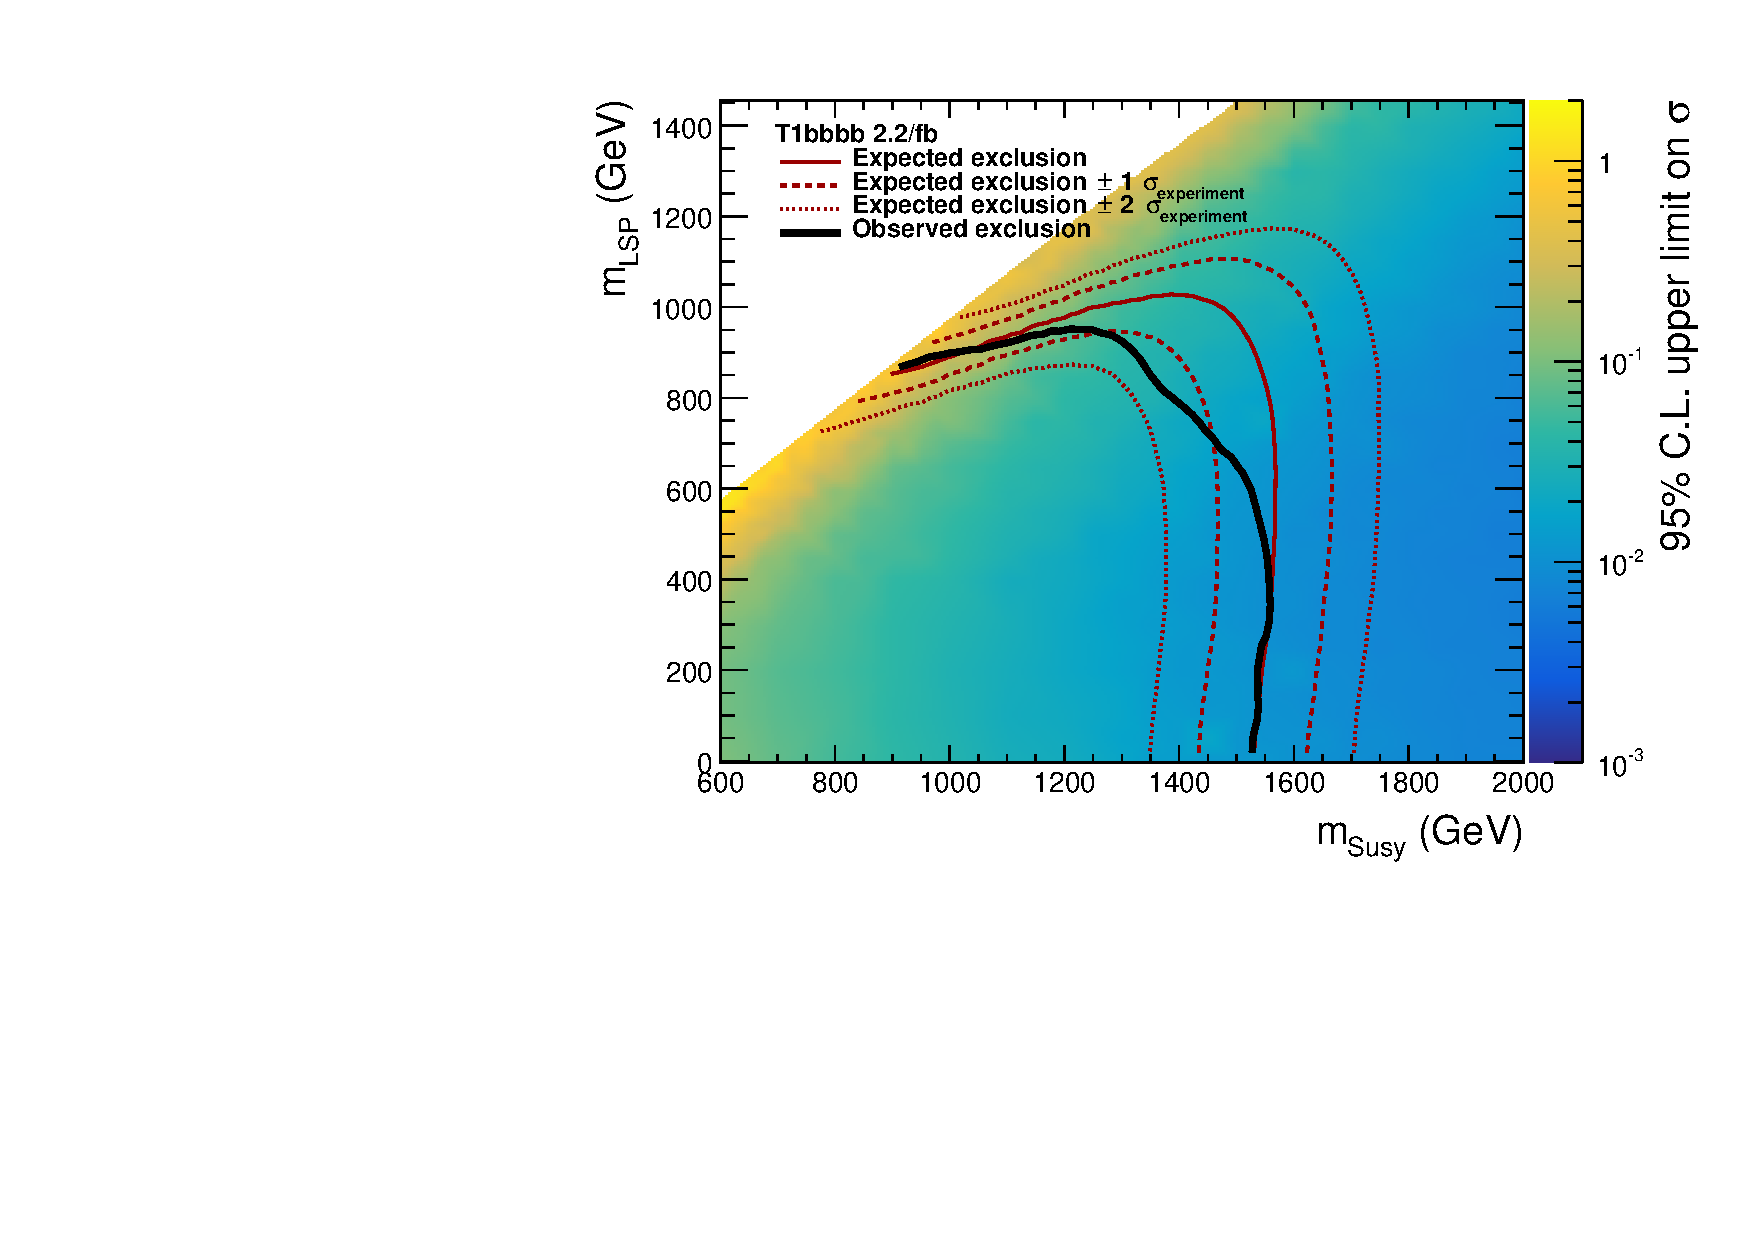
\includegraphics[width=0.32\linewidth]{T1bbbb.pdf}
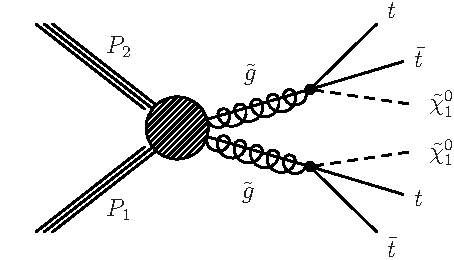
\includegraphics[width=0.32\linewidth]{T1tttt.pdf}
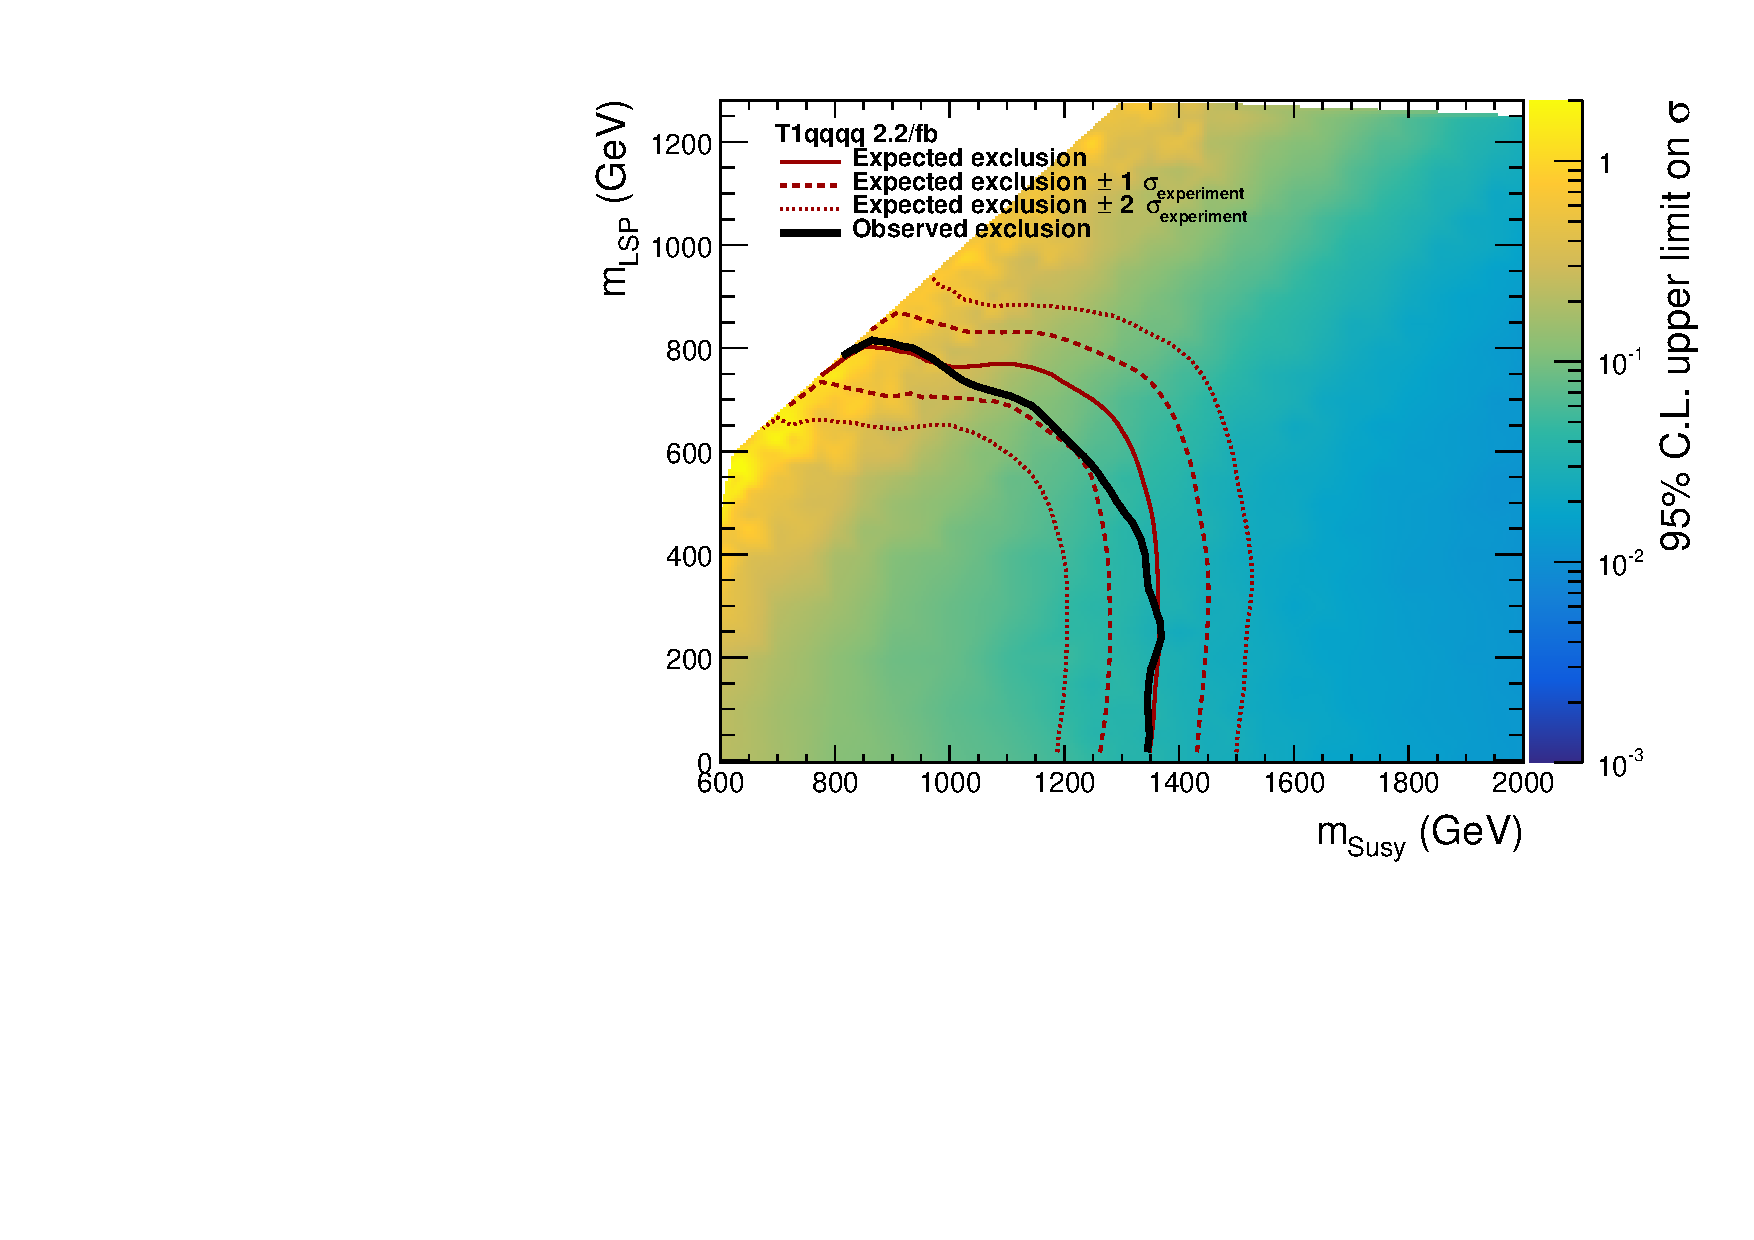
\includegraphics[width=0.32\linewidth]{T1qqqq.pdf}
\caption{
Feynman diagrams for the simplified models considered in the interpretation of this study.
}
\label{fig:feyn}
\end{figure*}

The search is devised around the kinematic variable \alphat that
provides powerful discrimination against multijet production, a
manifestation of quantum chromodynamics (QCD), and adheres to an
inclusive strategy with the aim of providing sensitivity to the widest
possible range of SUSY models. The \alphat variable is constructed from jet-based quantities to provide robust discriminating power between sources of genuine and misreconstructed missing energy, making it suitable for early searches.

The search is based on an examination
of the number of reconstructed jets per event, the scalar and vector sums of
transverse energies of these jets, and the number of these jets
identified as originating from bottom quarks. These
discriminating variables provide sensitivity to the different
production mechanisms of massive coloured sparticles at hadron
colliders (\ie squark-squark, squark-gluino, and gluino-gluino), a
large range of mass splittings between the parent sparticle and the
LSP, and third-generation squark signatures, respectively.

%%__________________________________________________________________||

\section{The CMS detector}
\label{sec:detector}

% Text copy/paste from https://twiki.cern.ch/twiki/bin/viewauth/CMS/Internal/PubDetector

The central feature of the CMS apparatus is a superconducting solenoid
of 6\unit{m} internal diameter, providing an axial magnetic field of
3.8\unit{T}. The bore of the solenoid is instrumented with several
particle detection systems. A silicon pixel and strip tracker measures
charged particles within the pseudorapidity~\cite{Chatrchyan:2008zzk}
range $\abs{\eta} < 2.5$.
%, where $\eta \equiv -\ln[\tan(\theta/2)]$ and $\theta$ is the polar
%angle of the trajectory of the particle with respect to the
%counterclockwise beam direction. 
A lead tungstate crystal electromagnetic calorimeter (ECAL), and a
brass and scintillator hadron calorimeter (HCAL), each composed of a
barrel and two endcap sections, extend over a pseudorapidity range
$\abs{\eta} < 3.0$. Outside the bore of the solenoid, forward
calorimeters extend the pseudorapidity coverage to $\abs{\eta} < 5.0$,
and muons are measured within $\abs{\eta} < 2.4$ by gas-ionization
detectors embedded in the steel flux-return yoke outside the
solenoid. A two-tier trigger system selects pp collision events of
interest. The first level (L1) of the trigger system, composed of
custom hardware processors, uses information from the calorimeters and
muon detectors to select the most interesting events in a fixed time
interval of less than 4\mus. The high-level trigger (HLT) processor
farm further decreases the event rate from around 100\unit{kHz} to
less than 1\unit{kHz}, before data storage. The CMS detector is nearly
hermetic, which allows for momentum-balance measurements in the plane
transverse to the beam axis. A more detailed description of the CMS
detector, together with a definition of the coordinate system used and
the relevant kinematic variables, can be found in
Ref.~\cite{Chatrchyan:2008zzk}.

%%__________________________________________________________________||
\section{Event reconstruction and selections} 
\label{sec:event_selection}

Global event reconstruction is provided by the particle-flow (PF)
algorithm~\cite{CMS-PAS-PFT-09-001, CMS-PAS-PFT-10-001}, which aims to
identify single candidate particles using an optimized combination of
information from all detector systems. In this process, the
identification of the particle type (photon, electron, muon, charged
hadron, neutral hadron) plays an important role in the determination
of the particle direction and energy.

In order to suppress SM processes with genuine \ptvecmiss from
neutrinos and select only multijet final states, events containing an
isolated electron~\cite{PAS-EGM-10-004} or muon~\cite{PAS-MUO-10-004}
with $\Pt > 10\GeV$ or isolated photon~\cite{PAS-EGM-10-006} with $\pt
> 25\GeV$ are vetoed. Furthermore, events containing an isolated track
with $\Pt > 10\gev$ are also vetoed in order to reduce the background
contribution from final states containing hadronically-decaying tau
leptons. Jets are reconstructed from candidate particles clustered by
the anti-$k_{\rm T}$ algorithm~\cite{antikt} with a size parameter of
$0.4$. The jet energies are corrected to account for the effects of
pileup and to establish a uniform relative response in $\eta$ and a
calibrated absolute response in transverse momentum
\pt~\cite{cms-jets}. Jets considered in the analysis are required to
have a transverse momentum above $40\gev$ and $|\eta| < 3$.

The mass scale of the physics processes being probed is characterised
by the scalar sum of the transverse momenta $\Pt$ of these jets,
defined as $\scalht = \sum_{i=1}^{N_{\rm jet}} \Pt^{\,\mathrm{j}_i}$,
where $N_{\rm jet}$ is the number of jets within the experimental
acceptance. The missing transverse momentum vector \ptvecmiss is
defined as the projection on the plane perpendicular to the beams of
the negative vector sum of the momenta of all candidate particles in
an event. Its magnitude is referred to as \ETmiss. The estimator for
\ETmiss used by this search is given by the magnitude of the vector
sum of the transverse momenta of these jets, $\mht =
|\sum_{i=1}^{N_\text{jet}} \ptvec^{\,\mathrm{j}_i}|$. Events are
vetoed if any additional jet satisfies $\Pt > 40\GeV$ and $|\eta| >
3$, in order to maintain the performance of the variable \mht as an
estimator of \ETmiss. Significant hadronic activity and \ptvecmiss in
the event is ensured by requiring $\scalht > 200\GeV$ and $\mht >
130\gev$, respectively. The most energetic jet in the event is
required to satisfy $\Pt > 100\gev$.

A number of beam- and detector-related effects can lead to events with
large values of \ETmiss, such as beam halo, reconstruction failures,
spurious detector noise, or event misreconstruction due to detector
inefficiencies. These events, with large, non-physical values of
\ETmiss, are rejected with high efficiency by applying a range of
dedicated vetoes~\cite{RA1Paper2012, cms-met}. An additional dedicated
veto is employed to deal with the circumstance in which several jets
with transverse momentum below the \Pt thresholds and collinear in
$\phi$ can result in significant \mht relative to \ETmiss, the latter
of which is less sensitive to jet thresholds. This type of background,
typical of multijet events, is suppressed while maintaining high
efficiency for SM or new physics processes with significant \ptvecmiss
by requiring $\mht / \ETmiss < 1.25$.

\begin{table*}[tb]
  \topcaption{Summary of the event selection requirements and
    categorisations used to define the signal region and control
    samples.}
  \label{tab:selections}
  \centering
  \footnotesize
  \begin{tabular}{ ll }
    \hline
    \multicolumn{2}{l}{\bf Baseline selection}\T\B                                                                                             \\
    \ETmiss cleaning             & Filters related to beam and instrumental effects                                                            \\ 
    Lepton/photon vetoes         & $\Pt > 10,\, 10,\, 25\GeV$ for isolated tracks, leptons, photons (respectively) and $\abs{\eta} < 2.5$      \\ 
    Jet $j_\text{i}$ acceptance  & Consider each jet $j_\text{i}$ that satisfies $\Pt^{j_\text{i}} > 40\GeV$ and $\abs{\eta^{j_\text{1}}} < 3$ \\
    Jet $j_\text{1}$ acceptance  & $\Pt^{j_\text{1}} > 100\GeV$ and $\abs{\eta^{j_\text{1}}} < 2.5$                                            \\
    Jet $j_\text{2}$ acceptance  & $\Pt^{j_\text{2}} < 40\GeV$ (monojet),                                                                      \\
                                 & $40 < \Pt^{j_\text{2}} < 100\GeV$ (asymmetric),                                                             \\
                                 & $\Pt^{j_\text{2}} > 100\GeV$ (symmetric)                                                                    \\
    Forward jet veto             & Veto events containing jet satisfying $\Pt > 40\GeV$ and $\abs{\eta} > 3$                                   \\
    Jets below threshold         & $\HTmiss / \ETmiss < 1.25$                                                                                  \\
    Energy sums                  & $\scalht > 200\GeV$ and $\HTmiss > 130\GeV$ \B                                                              \\
    \hline
    \multicolumn{2}{l}{\bf Event categorisation}\T\B                                                                                           \\
    \njet                        & 1 (monojet); 2, 3, 4, $\geq$5 (asymmetric); 2, 3, 4, $\geq$5 (symmetric)                                    \\
    \nb                          & 0, 1, 2, $\geq$3 ($\nb \leq \njet$)                                                                         \\
    \scalht (GeV)                & 200, 250, 300, 350, 400, 500, 600, $>$800\GeV (some bins are dropped/merged \vs \njet) \B                   \\
    \hline
    {\bf Signal region (SR)}     & Baseline selection + \T\B                                                                                   \\
    QCD multijet rejection \quad & $\alphat > 0.65$, 0.60, 0.55, 0.53, 0.52, 0.52, 0.52 (mapped to \scalht bins in range 200--800\GeV)         \\
    QCD multijet rejection       & $\bdphi > 0.5$\B                                                                                            \\[0.5ex]
    \hline
    {\bf Control samples (CS)}   & Baseline selection + \T\B                                                                                   \\
    Multijet-enriched            & SR + $\HTmiss/\ETmiss > 1.25$ (inverted)                                                                    \\  
    \gj                          & 
    1$\gamma$ with $\Pt > 200\GeV$, $\abs{\eta} < 1.45$, 
    $\Delta R(\gamma,j_{\text{i}}) > 1.0$, 
    $\scalht > 400\GeV$, same \alphat req. as SR                                                                                               \\[0.5ex]
    \mj                          & 
    1$\mu$ with $\Pt > 30\GeV$, $\abs{\eta} < 2.1$, 
%    $I^{\mu}_\text{rel} < 0.1$, 
    $\Delta R(\mu,j_{\text{i}}) > 0.5$,
    $30 < m_\text{T}(\ptvec^\mu,\ptvecmiss) < 125\GeV$                                                                                         \\[0.5ex]
    \mmj                         & 
    2$\mu$ with $\Pt > 30\GeV$, $\abs{\eta} < 2.1$, 
%    $I^{\mu}_\text{rel} < 0.1$, 
    $\Delta R(\mu_{1,2},j_{\text{i}}) > 0.5$, 
    $ \abs{m_{\mu\mu} - m_\text{Z}} < 25\GeV$ \B                                                                                               \\[0.5ex]
    \hline
  \end{tabular}
\end{table*}

The aforementioned selection requirements define a baseline set, as
summarised in Table~\ref{tab:selections}. Additional requirements,
described below, are utilised to define a sample of candidate signal
events, labelled henceforth as the signal region. Four additional
control samples of events are employed to estimate the background
contributions from SM processes, which modify and expand on the
baseline selection requirements. The first control sample is enriched
in multijet events and is used to estimate the multijet contribution
in the signal region. Three additional control samples comprising \gj,
\mj, or \mmj events, defined by the baseline set of selections and the
inversion of one of the photon or lepton vetoes, are used to estimate
background contributions from SM processes, predominantly \wlj,
\znunuj, and \ttbar production, that lead to final states containing
jets and significant \ptvecmiss. Additional kinematic requirements are
employed to ensure the control samples are enriched in the same SM
processes that contribute to background events in the signal region,
and are depleted in contributions from multijet production or a wide
variety of SUSY models (\ie so-called signal contamination).  The
control samples are defined such that the kinematic properties of
events in the control regions and the candidate signal events resemble
as closely as possible one another, once the photon, muon, or dimuon
system is ignored in the calculation of quantities such as \scalht and
\HTmiss. The event selection requirements for the four control samples
are summarised in Table~\ref{tab:selections}.

Events containing at least two jets are categorised according to {\it
  symmetric} or {\it asymmetric} topologies if the second-most
energetic jet satisfies, respectively, $\Pt > 100\gev$ or $40 < \Pt <
100\gev$. Events that contain only one jet satisfying the requirement
$\Pt > 40\gev$ are categorised as a {\it monojet} topology. The
symmetric topology targets the pair production of sparticles and their
cascade decays, while the monojet and asymmetric topologies target
nearly mass-degenerate SUSY models, as well as the direct production
of weakly interacting massive particles. Events are further
categorised according to the number of jets per event (\njet), the
number of reconstructed jets identified as originating from a b quark
(\nb), and \scalht. These categorisations, summarised in
Table~\ref{tab:selections}, are used identically for the signal region
and the four control samples. Finally, the search exploits the use of
the \mht variable as a discriminant between the dominant SM
backgrounds and new-physics signatures. The expected distribution of
events as a function of \mht is determined from simulation, an
approach that is validated in multiple data control samples.

For events satisfying the baseline selections described above,
summarised in Table~\ref{tab:selections}, the multijet background
dominates over all other SM backgrounds. The \alphat kinematic
variable, first introduced in Refs.~\cite{Randall:2008rw, RA1Paper},
is used to efficiently reject multijet events with transverse momentum
mismeasurements while retaining sensitivity to new physics with
genuine \ptvecmiss signatures. The variable \alphat depends solely on
the measurements of the transverse momenta and azimuthal angles of
jets and it is intrinsically robust against the presence of jet energy
mismeasurements in multijet systems. For dijet events, the \alphat
variable is defined as $\alphat = \Pt^{\rm j_2}/M_\text{T}$ where
$\Pt^{\rm j_2}$ is the transverse momentum of the less-energetic jet,
and $M_\text{T}$ is the transverse mass of the dijet system.  For a
perfectly measured dijet event with $\Pt^{\mathrm{j}_1} =
\Pt^{\mathrm{j}_2}$ and jets back-to-back in $\phi$, and in the limit
in which the momentum of each jet is large compared with its mass, the
value of \alphat is 0.5. For the case of an imbalance in the measured
transverse momenta of back-to-back jets, \alphat is reduced to a value
smaller than 0.5, which gives the variable its intrinsic
robustness. Values significantly greater than 0.5 are observed when
the two jets are not back to back and are recoiling against
significant, genuine \ptvecmiss. The definition of the \alphat
variable can be generalised for events with two or more jets, as
described in Ref.~\cite{RA1Paper2012}.

Multijet events typically populate the region $\alphat \lesssim 0.5$
and the \alphat distribution is characterised by a sharp edge at 0.5,
beyond which the multijet event yield falls by several orders of
magnitude. Multijet events with extremely rare but large stochastic
fluctuations in the calorimetric measurements of jet energies can lead
to values of \alphat slightly above 0.5. The edge at 0.5 sharpens with
increasing \scalht for multijet events, primarily due to a
corresponding increase in the average jet energy and thus an
improvement in the jet energy resolution, but also because the
threshold effect of jets below the \Pt threshold contributing
significantly to \mht decreases with increasing \scalht. This
motivates a \scalht-dependent \alphat requirement that varies in the
range 0.52--0.65 for the region $\scalht < 800\gev$.

The \dphi variable considers the minimum azimuthal angular separation
of a jet and the \mht vector derived from all other jets in the
event. The \dphi variable provides powerful discriminating power
between final states with genuine \ptvecmiss and mismeasured QCD
multijet events. The variable is also highly efficient at suppressing
any potential contribution from rare energetic multijet events that
yield high jet multiplicities and significant \ETmiss due to
high-multiplicity neutrino production in semileptonic heavy-flavour
decays. The neutrinos are typically collinear with respect to the axis
of a jet and carry a significant fraction of the energy. The
requirement $\dphi > 0.5$ is sufficient to suppress effectively the
multijet background. For the region $\scalht < 800\gev$, the
requirements on both the \alphat and \dphi variables are utilised,
whereas for the region $\scalht > 800\gev$, the necessary control of
the QCD multijet background is achieved solely with the \dphi
requirement.

The tight requirements on the variables \alphat, \dphi, and
\HTmiss/\ETmiss suppress the expected contribution from multijet
events to the percent level with respect to the total expected
background counts from other SM processes, for all bins of the signal
region. Further, control variables are inspected to provide confidence
that any multijet contamination due to instrumental effects is
negligible. The aforementioned requirements complete the definition of
the signal region, and are summarised in Table~\ref{tab:selections}.

%Figure~\ref{fig:alphat-bdphi} shows the \alphat and \dphi
%distributions observed in data for events that satisfy all other
%signal region selection criteria plus $\scalht > 300\gev$ and $\scalht
%> 800\gev$, respectively. In the case of the \alphat distribution, the
%events that satisfy $\alphat < 0.55$ must only fulfill the baseline
%selection criteria defined in Table~\ref{tab:selections}, no \mht
%requirement is made, and the events are recorded with an unbiased set
%of trigger \scalht conditions.

%\begin{figure*}[tbhp]
%  \begin{center}
%    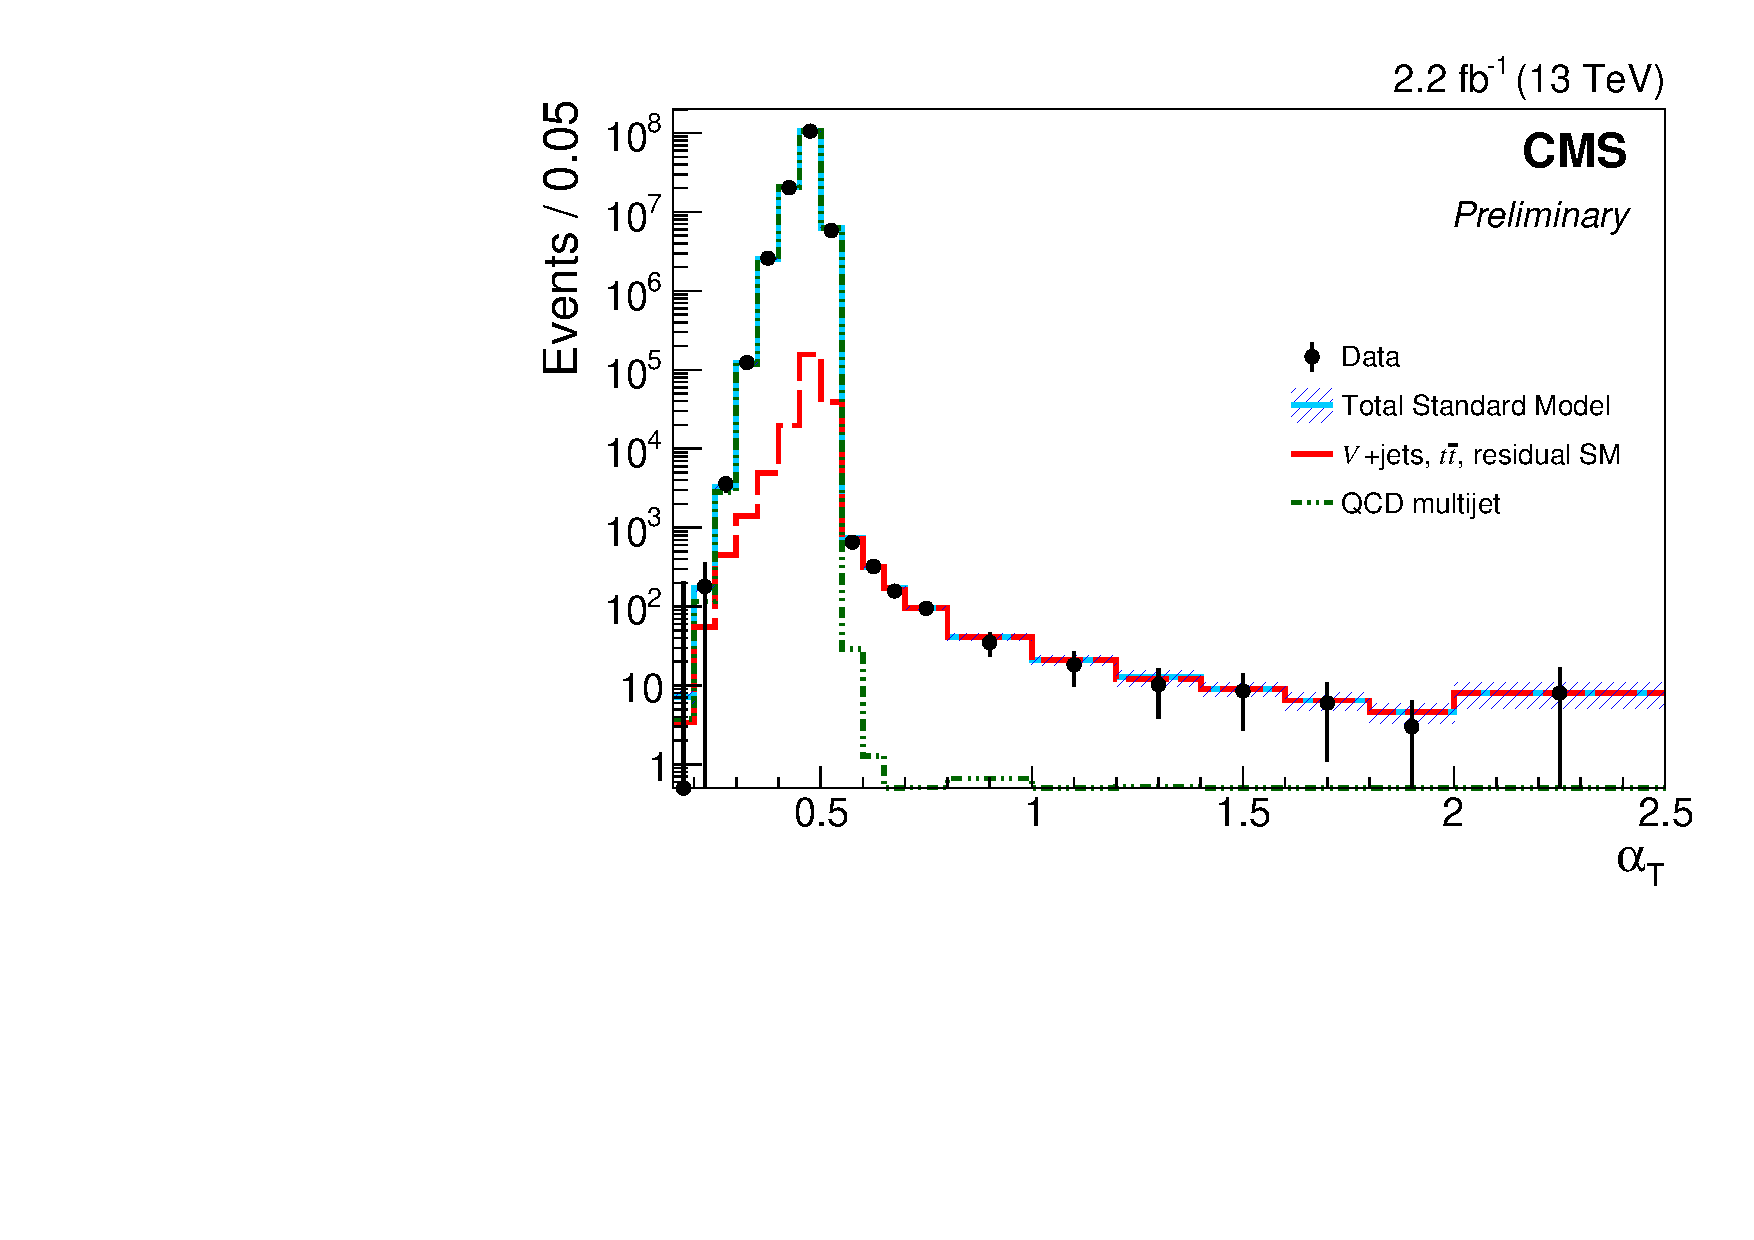
\includegraphics[width=0.49\textwidth]{alphaT_v4} \,
%    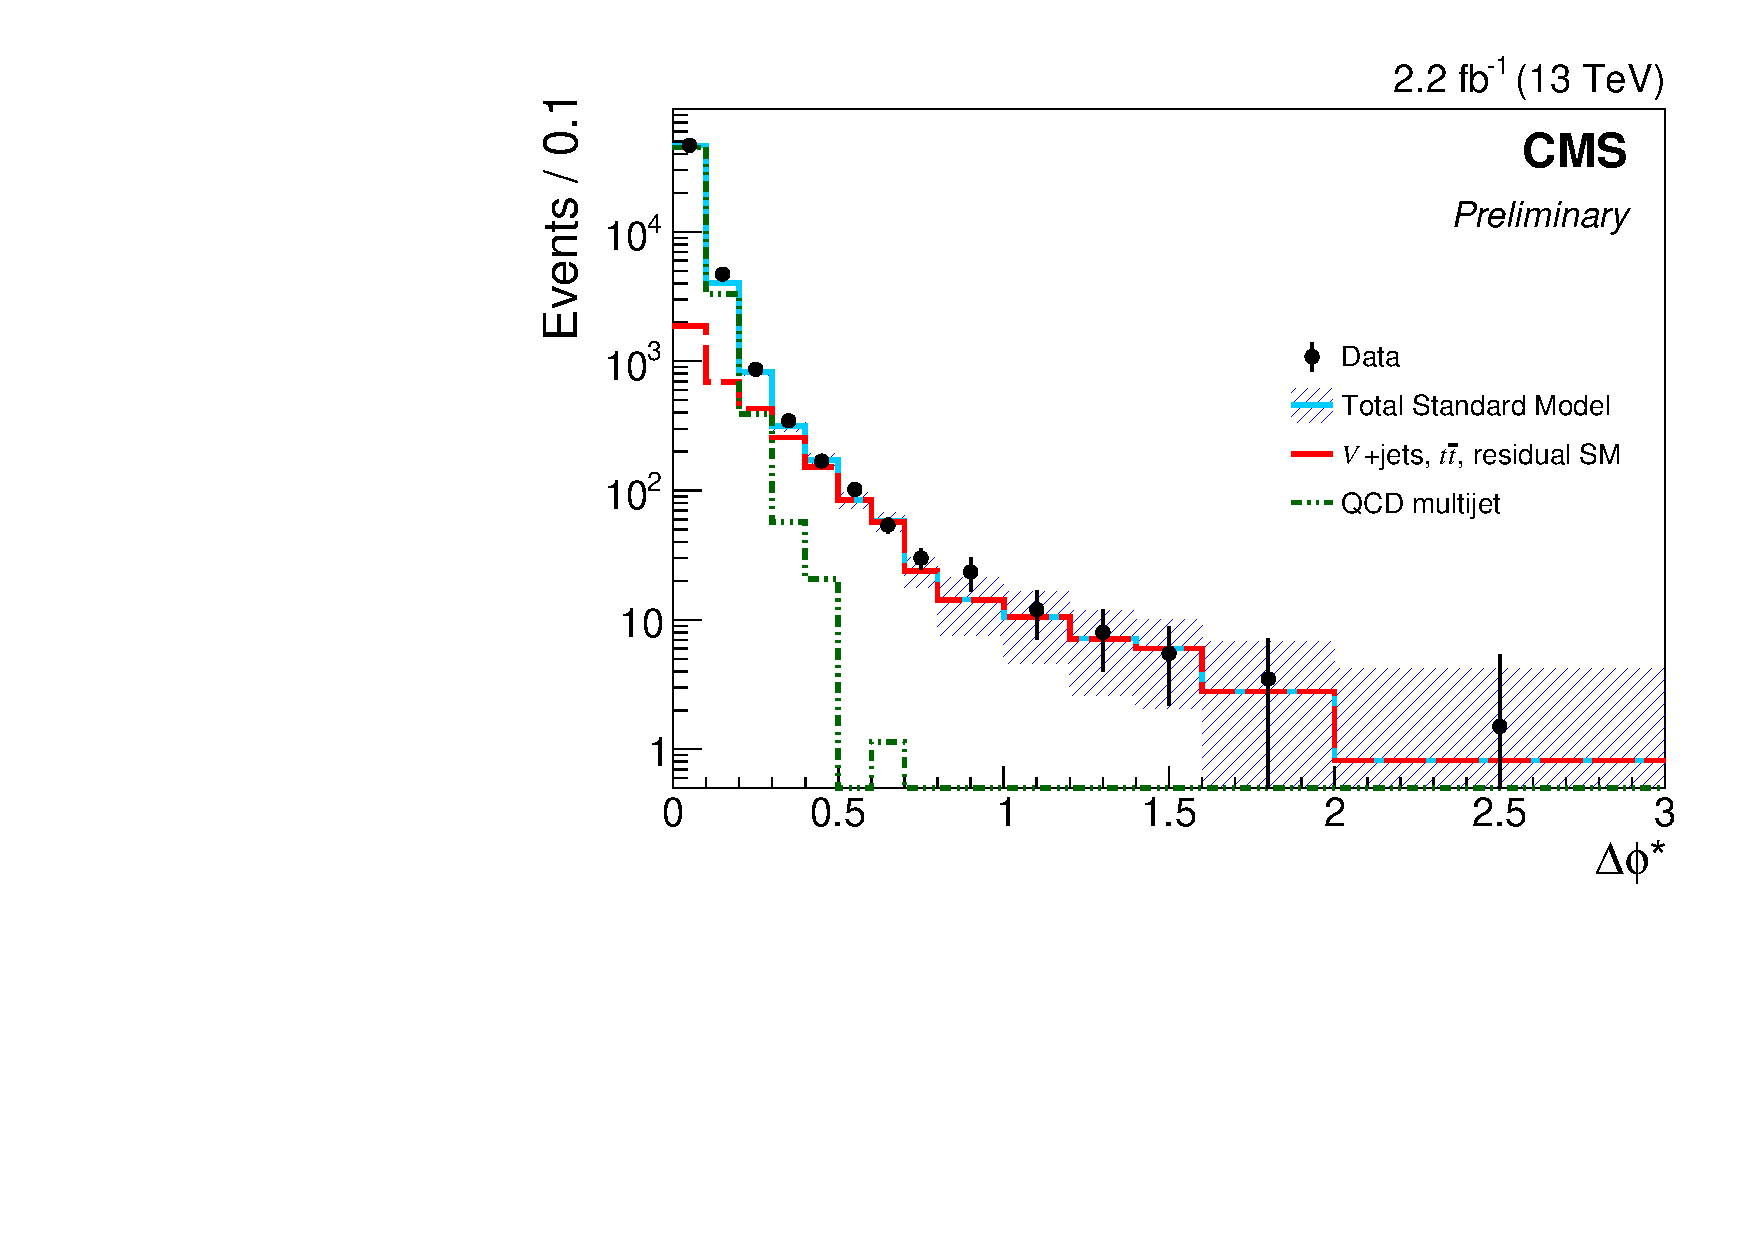
\includegraphics[width=0.49\textwidth]{bDPhi_v4} \\
%  \end{center}
%  \caption{(Left) The \alphat distribution observed in data for events
%    that are recorded with unbiased trigger conditions and satisfy the
%    baseline (full signal region) selection criteria for the region
%    $\alphat < 0.55$ ($\alphat > 0.55$). (Right) The \dphi
%    distribution observed in data for events that satisfy the full
%    signal region selection criteria and $\scalht > 800\gev$.  The
%    distributions for the QCD multijet backgrounds are determined from
%    simulation while all other SM backgrounds are estimated using a
%    $\mu$ + jets data control sample. %The uncertainties in the SM
%    %expectation are dominated by the statistical uncertainties 
%    %associated with the limited sample of simulated multijet events.
%    \label{fig:alphat-bdphi} 
%  }
%\end{figure*}

The categorisation of candidate signal events, as a function of \njet,
\nb, \scalht, and \HTmiss, and the number of bins within the signal
region are determined primarily by the statistical power of the
multiple data control samples. The signal region and control samples
cover a large phase space, defined primarily by the loose requirements
$\scalht > 200\GeV$ and $\HTmiss > 130\GeV$, and candidate signal
events are categorised into 194 exclusive sub-regions according to
\njet, \nb, and \scalht. Within each sub-region, events are further
categorised according to \HTmiss: the first bin is defined by the
range $130 < \HTmiss < 200\GeV$, subsequent bins have a width of
100\GeV, up to a final open bin that satisfies $\HTmiss > 800\GeV$. If
the statistical power of the simulated or data control samples is
limited, the higher \HTmiss bins are merged, reducing the threshold on
the final open bin, to the limiting case of a single open bin defined
by $\HTmiss > 130\GeV$. This procedure ensures the information taken
from simulation is always adequately supported by checks in the data
control samples. On average, less than four bins in \HTmiss are
utilised per (\njet, \nb, \scalht) category.

Candidate signal events are recorded with multiple jet-based trigger
conditions that require both \scalht and \alphat to satisfy
predetermined thresholds. In addition, a trigger condition based
solely on \scalht is used to record candidate events for the region
$\scalht > 800\gev$. A dedicated trigger condition requiring the
presence of significant \mht and \ETmiss is used to record events
containing one or more jets. The trigger-level jet energies are
corrected to account for energy scale and pileup effects. The trigger
strategy provides efficiencies at or near 100\% for all bins of the
signal region.

\section{Estimation of backgrounds}
\label{sec:backgrounds}

\subsection{Multijet background}
\label{sec:qcd_background}

The signal region is defined in a manner that suppresses the expected
contribution from multijet production to the percent level with
respect to the total expected background from other SM processes for
all signal region bins.
% all event categories, defined in terms of \njet and \nb, and all
% bins, defined in \scalht and \HTmiss. 
This is achieved primarily through the application of very tight
requirements on the variables \alphat and \dphi, as described in
Section~\ref{sec:signal_region}, as well as the requirement $\mhtmet <
1.25$. In this section, we discuss these requirements further, and
present the estimate of the suppression of the multijet background.

%The contamination from multijet events in the signal region is
%estimated using a multijet-enriched data sideband to the signal
%region, defined by the (inverted) requirement $\mhtmet > 1.25$. The
%observed counts in data are categorised according to \njet and \scalht
%and are corrected to account for contamination from vector boson and
%\ttbar production, and residual contributions from other SM processes,
%which are estimated using the \mj control region with the method
%described in Section~\ref{sec:ewk_background}. 
%The corrected data counts $\mathcal{N}^\text{data}(\njet, \scalht)$
%are used to estimate the multijet background in the signal region
%$\mathcal{P}(\njet, \scalht)$ through multiplication with the ratio
%$\mathcal{R}^\text{QCD}(\njet, \scalht)$ of multijet events that
%satisfy the requirement $\mhtmet < 1.25$ to those that fail, which is
%determined independently for events categorised according to \njet and
%\scalht from simulation. 
%Finally, the differential distribution of $\mathcal{P}(\njet,
%\scalht)$ as a function of \nb and \HTmiss is described by the
%multiplier term $\mathcal{K}_{\njet, \scalht}(\nb, \HTmiss)$, which is
%assumed to exhibit the same distribution as the nonmultijet
%backgrounds, as determined from simulation.

The contamination from multijet events in the signal region is
estimated using a multijet-enriched data sideband to the signal
region, defined by the (inverted) requirement $\mhtmet > 1.25$. The
observed counts in data, categorised according to \njet and \scalht,
are corrected to account for contamination from nonmultijet SM
processes, and the corrected counts $\mathcal{N}^\text{data}(\njet,
\scalht)$ are assumed to arise solely from QCD multijet
production. The nonmultijet processes, which comprise vector boson
and \ttbar production and residual contributions from other SM
processes, are estimated using the \mj control region, as 
described in Section~\ref{sec:ewk_background}. 

%Independent ratios $\mathcal{R}^\text{QCD}(\njet, \scalht)$ of
%multijet events that satisfy the requirement $\mhtmet < 1.25$ to those
%that fail, where the events are categorised according to \njet and
%\scalht, are determined from simulation.
Independent ratios $\mathcal{R}^\text{QCD}(\njet, \scalht)$ of the
number of multijet events that satisfy the requirement $\mhtmet <
1.25$ to the number that fail are determined from simulation for
events categorised according to \njet and \scalht, and inclusively
with respect to \nb and \HTmiss. The product of each ratio
$\mathcal{R}^\text{QCD}(\njet, \scalht)$ and the corresponding
corrected data count $\mathcal{N}^\text{data}(\njet, \scalht)$
provides the estimate of the multijet background $\mathcal{P}(\njet,
\scalht)$. The distributions of the predicted event counts
$\mathcal{P}(\njet, \scalht)$ as a function of \nb and \HTmiss are
implemented with the multiplier terms $\mathcal{K}_{\njet,
  \scalht}(\nb, \HTmiss)$, and are assumed to be identical to the
distributions expected for the nonmultijet backgrounds. This final
assumption is based on studies in simulation and is a valid
approximation given the magnitude of the statistical and systematic
uncertainties in the ratios $\mathcal{R}^\text{QCD}(\njet, \scalht)$,
as described below.
%Each estimate is assumed to distribute identically to the
%nonmultijet backgrounds as a function of \nb and \HTmiss. This final
%assumption, implemented by the multiplier term $\mathcal{K}_{\njet,
%  \scalht}(\nb, \HTmiss)$, is based on studies in simulation. Hence
%$\mathcal{K}_{\njet,\scalht}(\nb, \HTmiss) = 1$, which is a valid
%approximation given the magnitude of the uncertainties in the ratios
%$\mathcal{R}^\text{QCD}(\njet, \scalht)$, as described below.
Assuming $i$, $j$, $k$, and $l$ are the bin indices for, respectively,
\njet, \scalht, \nb, and \HTmiss:

\begin{equation}
  \label{eq:qcd}
  \mathcal{P}( i, j, k, l ) =
  \mathcal{N}^\text{data}( i, j )\;
  \mathcal{R}^\text{QCD}( i, j )\;
  \mathcal{K}_{i,j}( k, l ).
\end{equation}

\begin{figure}[!t]
  \begin{center}
%    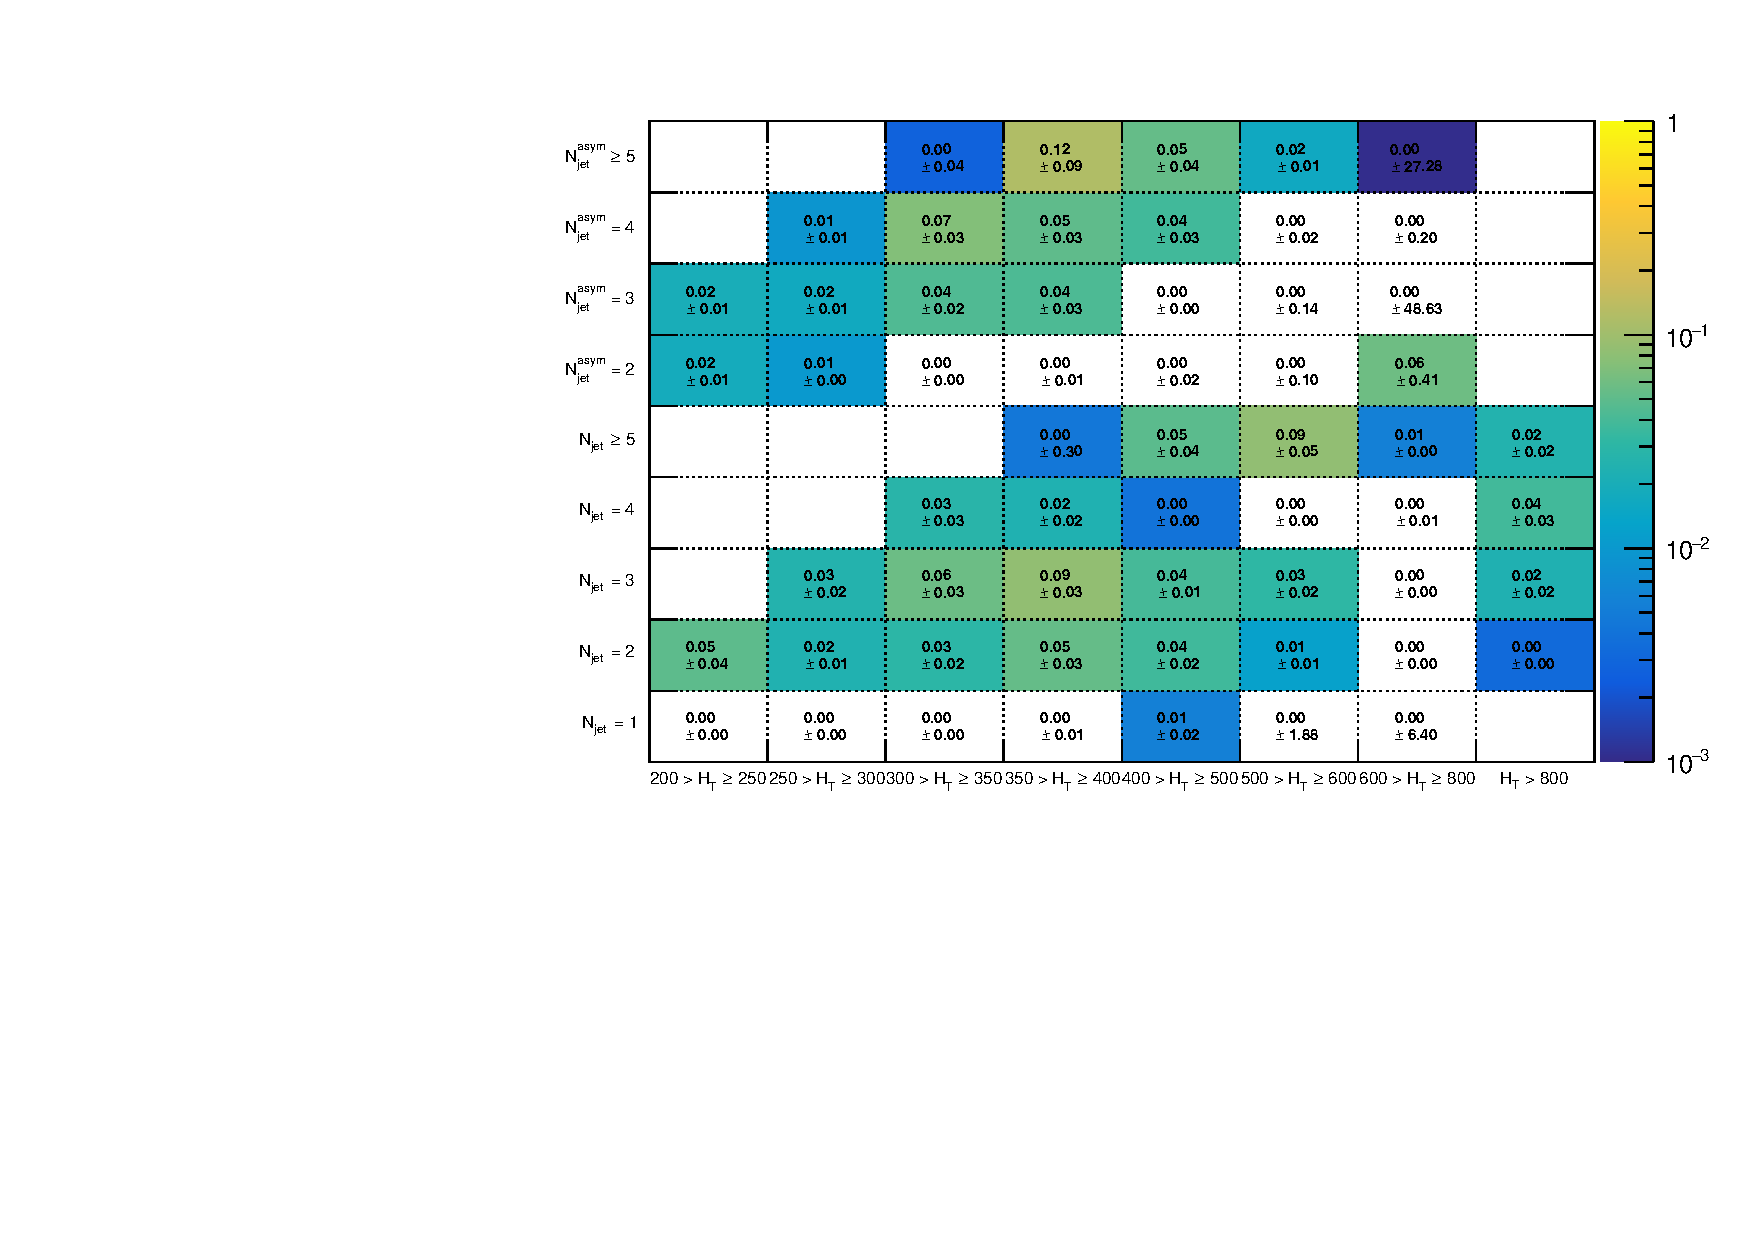
\includegraphics[width=0.49\textwidth]{figures/qcd/v0/qcd_pred} \,
    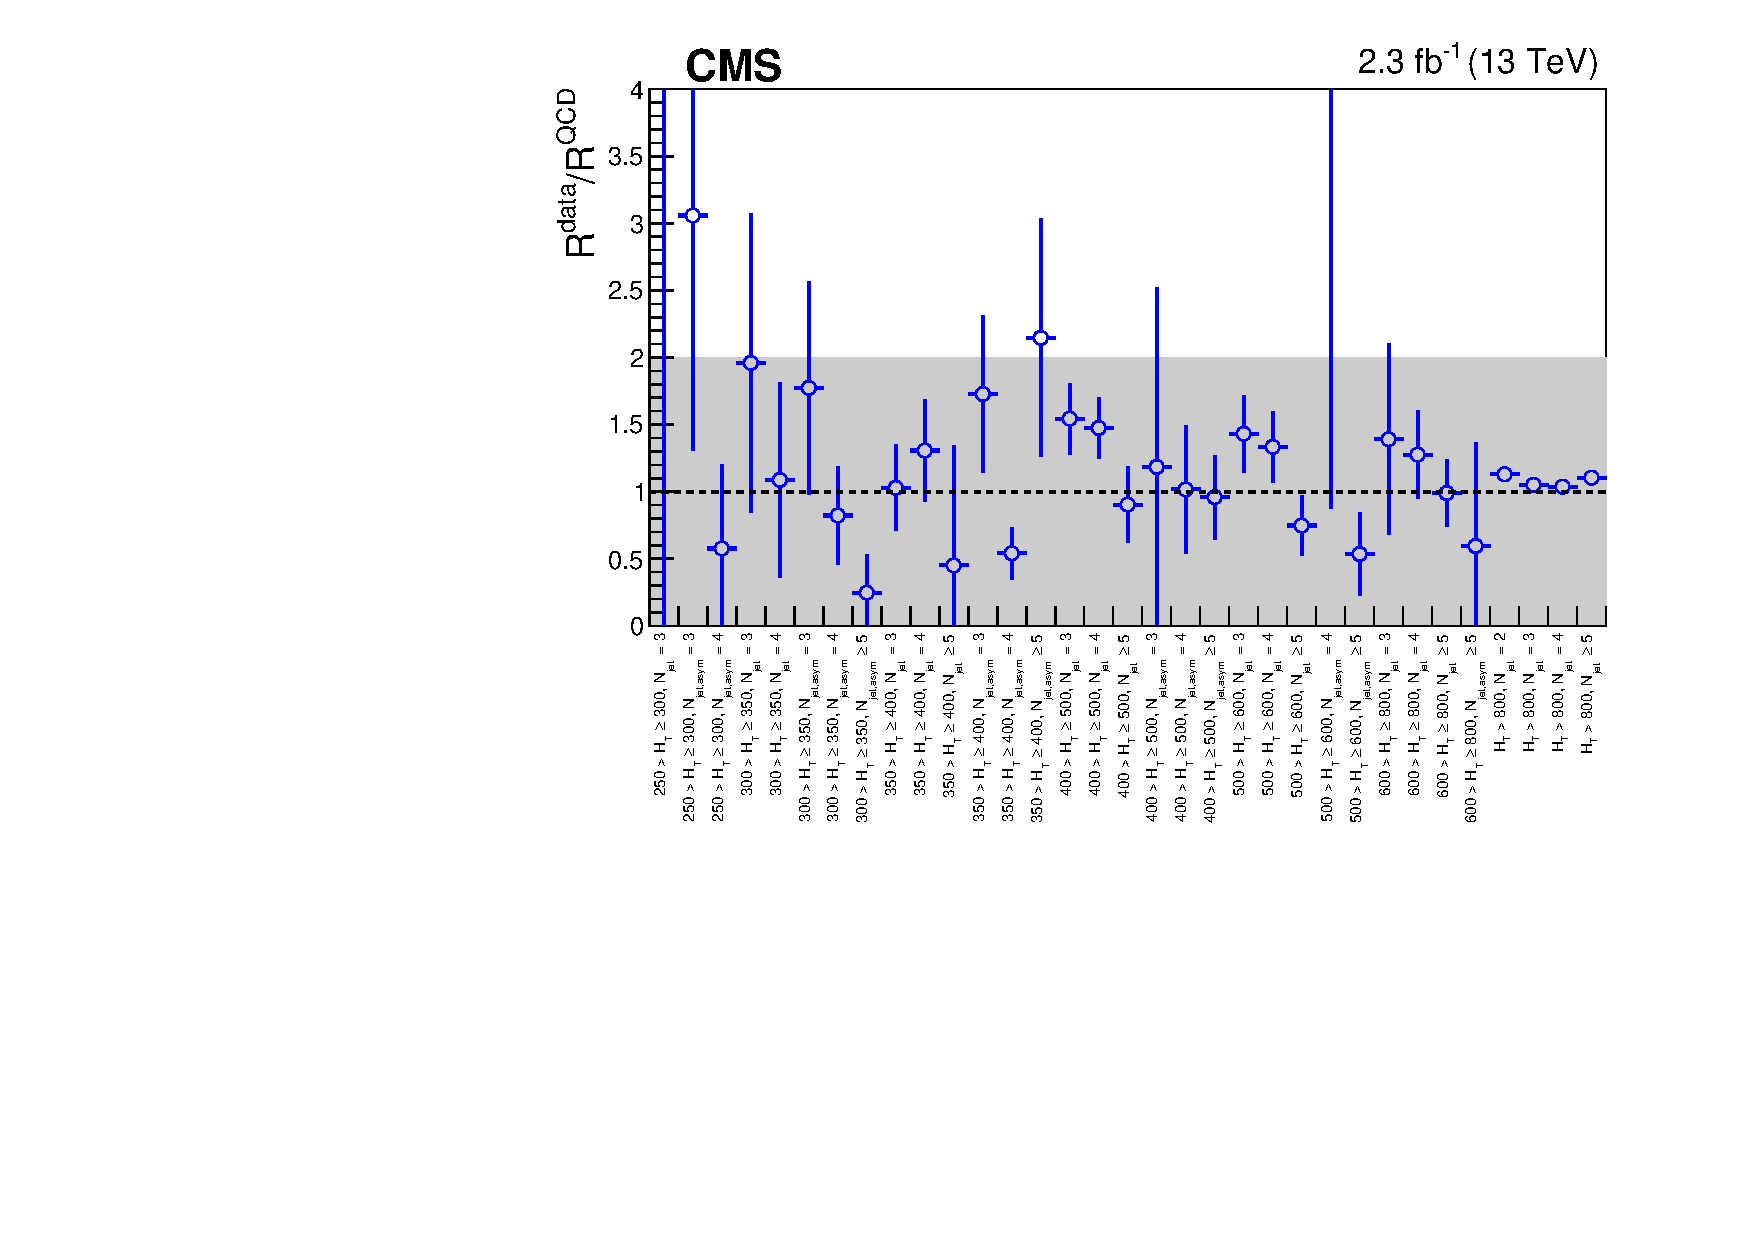
\includegraphics[width=0.7\textwidth]{figures/qcd/v1/DoubleRatioQCD_noEmpty} \\
  \end{center}
  \caption{Validation of the ratio $\mathcal{R}^\text{QCD}$ determined
    from simulation in bins of \njet and \scalht by comparing with an
    equivalent ratio $\mathcal{R}^\text{data}$ constructed from data 
    in a multijet-enriched sideband to the signal region. A value of
    unity is expected for the double ratio $\mathcal{R}^\text{data} /
    \mathcal{R}^\text{QCD}$, and the grey shaded band represents the
    assumed systematic uncertainty of 100\% in
    $\mathcal{R}^\text{QCD}$. 
  }
  \label{fig:qcd} 
\end{figure}

The use of simulation to determine $\mathcal{R}^\text{QCD}(\njet,
\scalht)$ is validated using a multijet-enriched data sideband defined
by $\bdphi < 0.5$.
%and an \alphat requirement identical to that used for the signal
%region, which is dependent on the value \scalht, as summarised in
%Table~\ref{}. 
Each ratio $\mathcal{R}^\text{data}(\njet, \scalht)$ is constructed
from data counts, corrected to account for contributions from
nonmultijet processes, and compared with the corresponding ratio
$\mathcal{R}^\text{QCD}(\njet, \scalht)$, determined from simulation,
through the double ratio
$\mathcal{R}^\text{data}/\mathcal{R}^\text{QCD}$, as shown in
Fig.~\ref{fig:qcd}. The double ratios are observed to be close to, or
statistically compatible with, unity across the full phase space of
the signal region, including the bins at high \scalht, which exhibit
the highest statistical precision. In addition to statistical
uncertainties as large as $\sim 100\%$, a systematic uncertainty of
100\% in $\mathcal{R}^\text{QCD}$ is assumed to adequately cover the
observed level of agreement for the full signal region phase space, as
well as any limitations in the assumptions concerning
$\mathcal{K}_{\njet, \scalht}(\nb, \HTmiss)$ for all event categories
defined in terms of \njet and \scalht.

%Finally, data control variables, such as $\bdphimod$, are inspected
%for localised populations in $(\eta,\phi)$-space to provide confidence
%that any multijet contamination due to instrumental effects is
%negligible.

%%__________________________________________________________________||
\section{Estimation of SM backgrounds with genuine \ptvecmiss}
\label{sec:ewk_background}

Following the suppression of multijet events, the background counts in
the signal region mainly arise from SM processes that produce
neutrinos, resulting in final states with significant \ptvecmiss. In
events with low counts of jets and b quark jets, the largest
backgrounds with genuine \ptvecmiss are from the associated production
of W or Z bosons with jets, followed by either the weak decays \znunu
or \wtaunu, where the $\tau$ decays hadronically and is identified as
a jet; or by leptonic decays that are not rejected by the dedicated
electron or muon vetoes. The veto of events containing isolated tracks
is efficient at further suppressing these backgrounds as well as the
single-prong hadronic decay of the tau lepton. At higher jet and b-tag
multiplicities, top quark production followed by semileptonic weak top
quark decay becomes important.

The simulated samples of \gj, \wlj, \zllj, and \ttbar production are
normalised to data using scale factors derived in data sidebands,
enriched in the relevant process. The definition of the sidebands, the
selection applied and the scale factors are listed in
Table~\ref{tab:sideband-corrs}. These factors are derived after all
other corrections are applied to the simulated samples.

\begin{table}[!h]
  \footnotesize
  \centering
  \topcaption{Cross section corrections for SM processes determined from
    data sidebands.}
  \label{tab:sideband-corrs}
  \begin{tabular}
    {lllc}
    \hline
    SM process & Control sample & Data sideband           & Corrrection\T\B   \\
    \hline                   
    \gj        & \gj            & $0.50 < \alphat < 0.52$ & $1.33 \pm 0.03$\T \\
    \wlj       & \mj            & $100 < \mht < 130\GeV$  & $1.13 \pm 0.01$   \\
    \zllj      & \mmj           & $100 < \mht < 130\GeV$  & $0.99 \pm 0.02$   \\
    \ttbar     & \mj, \mmj      & $100 < \mht < 130\GeV$  & $0.86 \pm 0.01$\B \\
    \hline
  \end{tabular}
\end{table}

The method to estimate the non-multijet backgrounds in the signal
region relies on the use of transfer factors, which are constructed
per bin (in terms of \njet, \nb, and \scalht) per data control
sample. The transfer factors are determined from the simulated event
samples and are ratios of expected yields in the corresponding bins of
the signal region and control samples. The transfer factors are used
to extrapolate from the event yields measured in data control samples
to an expectation for the total background event yields in the signal
region.  Three disjoint data control samples, binned identically to
the signal region, are used to estimate the contributions from the
non-multijet SM background processes, as summarised in
Table~~\ref{tab:selections}.

The \mj sample is recorded using a trigger condition that requires an
isolated muon and the event selection criteria are chosen in order to
ensure high trigger efficiency. Furthermore, the muon is required to
be well separated from the jets in the event and the transverse mass
($m_{\text{T}}$) of the muon and \ptvecmiss system must satisfy $30 <
m_\text{T}(\ptvec^\mu,\ptvecmiss) < 125\GeV$ to ensure a sample rich
in W bosons (produced promptly or from the decay of top quarks). The
\mmj sample uses similar selection criteria as the \mj sample and the
same trigger condition. Exactly two oppositely-charged, isolated muons
are required, the muons must be distanced from the jets in the event,
and the invariant mass of the dimuon system ($m_{\mu\mu}$) must be
within a window of $\pm 25\GeV$ around the mass of the Z boson, $
\abs{m_{\mu\mu} - m_\text{Z}} < 25\GeV$. For both the muon and dimuon
samples, no requirement is made on the variable \alphat in order to
increase the statistical precision of the predictions derived from
these samples, in contrast to the identical \alphat requirements made
for the signal region and photon control sample. The \gj sample is
recorded using a single photon trigger condition. The event selection
criteria comprise an isolated photon with $\Et > 200\gev$ and $\scalht
> 400\GeV$.

Three independent estimates of the irreducible background of \znunu +
jets events are determined from the \gj, \mmj, and \mj data control
samples. The \gj and \zmumu + jets processes have similar kinematic
properties when the photon or muons are ignored~\cite{Bern:2011pa}, 
albeit different acceptances. In addition, the \gj process has a
larger production cross section than \znunu + jets events. The \mj
data sample is used to provide an estimate for the \znunu\ + jets
contribution as well as the other dominant SM processes, \ttbar and W
boson production. Residual contributions from processes such as
single-top-quark, diboson, and Drell-Yan production are also included.

\newcommand{\phh}{\ensuremath{\phantom{1-}}}
\begin{table*}[h!]
  \caption{
    Systematic uncertainties in the transfer factors used in
    the method to estimate the SM backgrounds with genuine \ptvecmiss
    in the signal region. The quoted ranges provide the minimum and
    maximum values used across all bins in \njet and \scalht.
  } 
  \label{tab:bkgd_systs}
  \centering
  \footnotesize
  \begin{tabular}{ lrrrr }
    \hline
    Systematic source         & \multicolumn{4}{c}{Uncertainty in transfer factor [\%]}\T\B \\
    \cline{2-5} 
                              & $\mj \Rightarrow \ttbar/\PW$ 
                              & $\mj \Rightarrow \znunu$ 
                              & $\mmj \Rightarrow \znunu$ 
                              & $\gj \Rightarrow \znunu$\T\B                                \\
    \hline                                                    
    \multicolumn{5}{l}{\it Corrections applied to simulation:}\T\B                          \\
    Jet energy scale          & 1--5  & 1--5  & 1--5  & 1--5                                \\
    b-tag efficiency / mistag & 1--5  & 1--5  & 1--5  & 1--5                                \\
    Lepton scale factors      & 1--3  & 1--3  & 1--3  & -                                   \\
    Pileup                    & 0--2  & 0--2  & 0--2  & 0--2                                \\
    Signal trigger efficiency & 1--2  & 1--2  & 1--2  & 1--2                                \\
    Muon trigger efficiency   & 2     & 2     & 2     & -                                   \\
    Photon trigger efficiency & -     & -     & -     & 1--2                                \\
    Top quark \Pt             & 1--10 & 1--30 & 1--10 & -                                   \\ 
    \multicolumn{5}{l}{\it Derived from closure tests in data:}\T\B                         \\
    W/Z ratio                 & -     & 4--15 & -     & -                                   \\
    Z/$\gamma$ ratio          & -     & -     & -     & 6--11                               \\
    W/\ttbar composition      & 4--30 & -     & -     & -                                   \\
    W polarisation            & 2--10 & 2--10 & -     & -                                   \\
    \alphat / \bdphi          & 3--30 & 3--30 & 3--30 & -\B                                 \\
    \hline
  \end{tabular}
\end{table*}

Several sources of uncertainty in the transfer factors are evaluated.
The most relevant effects are discussed below, and generally fall into
one of two categories. The first category concerns uncertainties in
``scale factor'' corrections applied to simulation, which are
determined using inclusive data samples that are defined by loose
selection criteria, to account for the mismodelling of theoretical and
experimental parameters. The second category concerns ``closure
tests'' in data that probe various aspects of the accuracy of the
simulation to model correctly the transfer factors in the phase space
of this search.

The uncertainties in the transfer factors are studied for variations
in scale factors related to: the jet energy scale, the efficiency and
misidentification probability of b quark jets, the efficiency to
identify or veto well-reconstructed, isolated leptons, and the
modelling of the transverse momentum of top quarks. %~\cite{}. 
A 5\% uncertainty in the minimum bias cross section is assumed and
propagated through to the reweighting procedure to account for
differences between the simulated and data-derived measurements of the
pileup distributions.  Uncertainties in the trigger efficiency
measurements are also propagated to the transfer factors.  The
aforementioned systematic uncertainties, resulting from variations in
scale factors, are summarised in Table~\ref{tab:bkgd_systs}, along
with representative magnitudes.  Each source of uncertainty is assumed
to vary with a fully correlated behaviour across the full phase space
of the signal and control regions.

Sources of additional uncertainty are determined from sets of
``closure tests'' based on data control
samples~\cite{RA1Paper2012}. Each set uses the observed event counts
in up to eight bins in \scalht for each of the nine \njet event
categories in one of the three independent data control samples, along
with the corresponding transfer factors determined from simulation, to
obtain a prediction of the observed yields in another control sample
(or, in one case, \nb event category). 
Each set of tests is designed to target a specific (potential) source
of bias in the simulation modelling that may introduce an \njet- or
\scalht-dependent source of systematic bias in the transfer
factors~\cite{RA1Paper2012}. Several sets of tests are performed. The
$\PZ/\gamma$ ratio determined from simulation is tested against the
same ratio measured using \zmmj events and the \gj sample. The
$\PW/\PZ$ ratio is also probed using the \mj and \mmj samples. A
further set probes the modelling of the relative composition between
\wlj and \ttbar events using \mj events containing exactly zero or one
more b-tagged jets, which represents a larger extrapolation in
relative composition than used in the search.  The effects of W
polarisation are probed by using \mj events with a positively charged
muon to predict those containing a negatively charged muon. Finally,
the accuracy of the modelling of the efficiencies of the \alphat and
\bdphi requirements are estimated using the \mj sample.

For each set of tests, the level of closure, which considers only
statistical uncertainties, is inspected to ensure no statistically
significant biases are observed as a function of the nine \njet
categories or the eight \scalht bins. In the absence of such a bias,
the level of closure is recomputed by integrating over either all
monojet and asymmetric topologies, or the symmetric \njet
categories. The level of closure and its statistical uncertainty are
combined in quadrature to determine additional contributions to the
uncertainties in the transfer factors. These uncertainties are
considered to be fully correlated between the monojet and asymmetric
topologies or the symmetric topology, and fully uncorrelated between
these two regions in \njet and \scalht bins. If the closure tests use
the \mmj sample, the level of closure is determined by additionally
integrating over pairs of adjacent \scalht bins. These uncertainties,
derived from the closure tests in data, are summarised in
Table~\ref{tab:bkgd_systs}, along with representative
magnitudes. These uncertainties are the dominant contribution to the
total uncertainty in the transfer factors, due to the limited number
of events in the data control samples.

Templates determined from simulation are used to predict the
background counts in the \mht dimension. Uncertainties in the scale
factor corrections applied to simulated events, as discussed above in
the context of transfer factors, are propagated as uncertainties in
the \HTmiss templates. Uncertainties in the trigger efficiency
measurements are also propagated to the \HTmiss templates. These
sources of uncertainty are assumed to vary with a correlated behaviour
across the full phase space of the signal region. Multiple data
control samples are used to evaluate the degree to which the
simulation describes the \mht distributions observed in data, and to
assign appropriate systematic uncertainties, which can be significant
($\sim$50--100\%) in the most sensitive \mht bins.  The \mht templates
from simulation are compared to the distributions observed in the
control samples, and inspected for trends, by assuming a linear
behaviour of the ratio of observed and simulated counts as a function
of \HTmiss. Linear fits are performed independently for each bin
defined by \njet, \nb, and \scalht. No significant biases or trends
are observed, given the statistical power of the control samples, and
systematic uncertainties are determined from the constrained fit
parameters. These uncertainties are treated as fully uncorrelated
between bins defined in terms of \njet, \nb, and \scalht, and also
with respect to the systematic uncertainties in in the transfer
factors, summarised in Table~\ref{tab:bkgd_systs}.

%%__________________________________________________________________||

\clearpage
%%__________________________________________________________________||
\section{Results}
\label{sec:interpretation}

A likelihood model of the observations in all data samples is used to
obtain a consistent prediction of the SM backgrounds and to test for
the presence of a variety of signal models.  In each bin of \scalht
for events in the same category of \njet and \nb, the observation is
modelled as a Poisson-distributed variable around the sum of the SM
expectation and a potential signal contribution (assumed to be zero in
the following discussion). The SM expectation is related to the
expected yields in the \mj, \mmj, and \gj control samples via transfer
factors derived from simulation. Likelihood functions describe the
yields in the \scalht bins of the \mj, \mmj, and \gj control samples
in the same category of \njet and \nb as the signal region. The
systematic uncertainties summarised in Table~\ref{tab:bkgd_systs} are
accommodated in the likelihood function by nuisance parameters, the
measurements of which are assumed to follow a log-normal
distribution. In the presence of a non-zero signal contribution, the
CL$_{\mathrm{s}}$ technique~\cite{read, Cowan:2010js} is used to
determine upper limits on production cross section using asymptotic
formulae.

The expected number of events from SM processes is determined from a
simultaneous fit to the signal region and up to three control
samples. The likelihood function is maximised over all fit parameters
under the SM-only hypothesis.
Tables~\ref{tab:predewkdata_sig_comb_mono}--\ref{tab:predewkdata_sig_comb_sym} 
summarise the observed yields and ``a priori'' and ``a posteriori'' SM
expectations for signal candidate events in the monojet, asymmetric,
and symmetric categories, respectively. No significant tension is
observed between the predictions and data in the signal region, which
is well described by the SM-only hypothesis.

\begin{table}[h!]
\scriptsize
\centering
\caption{
  Observed data counts, ``pre-fit'' and ``post-fit'' background expectations  
  for all the \scalht bins and \njet, \nb multiplicity in the monojet event category. 
  The uncertainties include statistical as well as systematic contributions. 
  \label{tab:predewkdata_sig_comb_mono}}  
\scalebox{0.85}{\begin{tabular}{lccccccccc}
	\hline\hline
                    &              & \multicolumn{8}{c}{\scalht (\gev)}                                                                                                                                    \\ 
                    & (\njet, \nb) & 200-250               & 250-300              & 300-350              & 350-400            & 400-500            & 500-600            & 600-800           & 800-$\infty$ \\ [0.8ex] 
\hline
 Data & $(1j,0)$ & $13094$ & $4130$ & $1477$ & $663$ & $461$ & $118$ & $50$ & -- \\[0.5ex]
 SM pre-fit & $(1j,0)$ & $12319.3\pm985.8$ & $4167.9\pm384.1$ & $1474.1\pm155.2$ & $559.8\pm95.2$ & $463.1\pm74.5$ & $145.6\pm29.1$ & $60.4\pm25.1$ & -- \\[0.5ex]
 SM post-fit & $(1j,0)$ & $13012.3\pm112.8$ & $4133.5\pm57.7$ & $1480.8\pm33.9$ & $638.0\pm21.4$ & $439.5\pm16.0$ & $118.1\pm7.0$ & $51.3\pm6.4$ & -- \\[0.5ex]
 Data & $(1j,1)$ & $475$ & $151$ & $57$ & $25$ & $24$ & $6$ & -- & -- \\[0.5ex]
 SM pre-fit & $(1j,1)$ & $505.3\pm64.3$ & $169.6\pm24.6$ & $61.3\pm10.3$ & $21.3\pm4.5$ & $21.0\pm4.4$ & $4.7\pm1.3$ & -- & -- \\[0.5ex]
 SM post-fit & $(1j,1)$ & $488.4\pm18.1$ & $157.9\pm11.0$ & $58.1\pm6.2$ & $24.1\pm3.8$ & $20.8\pm2.6$ & $5.3\pm1.4$ & -- & -- \\[0.5ex]

	\hline
	\hline
\end{tabular}}
\end{table}

\clearpage
\begin{table}[h!]
\scriptsize
\centering
\caption{
  Observed data counts, ``pre-fit'' and ``post-fit'' background expectations  
  for all the \scalht bins and \njet, \nb multiplicity in the asymmetric event category. 
  The uncertainties include statistical as well as systematic contributions. 
  \label{tab:predewkdata_sig_comb_asym}}  
\scalebox{0.85}{\begin{tabular}{lccccccccc}
	\hline\hline
                    &                   & \multicolumn{8}{c}{\scalht (\gev)}                                                                                                                              \\ 
                    & (\njet, \nb)      & 200-250              & 250-300              & 300-350            & 350-400            & 400-500            & 500-600          & 600-800          & 800-$\infty$ \\ [0.8ex] 
\hline

 Data & $(2a,0)$ & $5788$ & $1585$ & $584$ & $232$ & $139$ & $26$ & $16$ & -- \\[0.5ex]
 SM pre-fit & $(2a,0)$ & $5890.6\pm544.0$ & $1695.0\pm180.5$ & $601.3\pm65.1$ & $224.3\pm38.4$ & $144.4\pm25.0$ & $36.4\pm7.1$ & $21.0\pm8.1$ & -- \\[0.5ex]
 SM post-fit & $(2a,0)$ & $5831.5\pm81.6$ & $1621.6\pm35.0$ & $581.0\pm17.9$ & $227.5\pm9.5$ & $136.5\pm6.4$ & $30.0\pm2.6$ & $18.3\pm3.2$ & -- \\[0.5ex]
 Data & $(2a,1)$ & $536$ & $152$ & $51$ & $18$ & $7$ & $4$ & -- & -- \\[0.5ex]
 SM pre-fit & $(2a,1)$ & $543.8\pm62.0$ & $161.7\pm22.6$ & $49.3\pm7.7$ & $20.5\pm3.9$ & $12.9\pm2.6$ & $4.3\pm1.0$ & -- & -- \\[0.5ex]
 SM post-fit & $(2a,1)$ & $541.0\pm16.4$ & $153.8\pm7.1$ & $49.7\pm3.7$ & $19.7\pm2.2$ & $10.7\pm1.4$ & $4.0\pm1.0$ & -- & -- \\[0.5ex]
 Data & $(2a,2)$ & $31$ & $10$ & $3$ & $1$ & $0$ & -- & -- & -- \\[0.5ex]
 SM pre-fit & $(2a,2)$ & $29.7\pm4.0$ & $7.2\pm1.2$ & $6.5\pm1.2$ & $2.0\pm0.5$ & $0.8\pm0.2$ & -- & -- & -- \\[0.5ex]
 SM post-fit & $(2a,2)$ & $29.5\pm3.5$ & $7.4\pm1.2$ & $5.0\pm1.1$ & $1.8\pm0.6$ & $0.6\pm0.3$ & -- & -- & -- \\[0.5ex]
 Data & $(3a,0)$ & $1599$ & $1609$ & $777$ & $239$ & $95$ & $15$ & $9$ & -- \\[0.5ex]
 SM pre-fit & $(3a,0)$ & $1669.4\pm163.3$ & $1529.4\pm171.2$ & $822.9\pm127.9$ & $272.3\pm60.5$ & $111.3\pm18.2$ & $19.7\pm4.0$ & $9.3\pm4.1$ & -- \\[0.5ex]
 SM post-fit & $(3a,0)$ & $1624.8\pm39.6$ & $1561.5\pm44.5$ & $781.7\pm28.8$ & $258.7\pm13.4$ & $100.9\pm5.4$ & $16.5\pm1.7$ & $8.0\pm1.5$ & -- \\[0.5ex]
 Data & $(3a,1)$ & $340$ & $299$ & $152$ & $59$ & $15$ & $1$ & $1$ & -- \\[0.5ex]
 SM pre-fit & $(3a,1)$ & $340.3\pm38.6$ & $357.2\pm51.6$ & $156.6\pm28.2$ & $46.1\pm12.0$ & $14.6\pm2.7$ & $2.3\pm0.7$ & $1.1\pm0.5$ & -- \\[0.5ex]
 SM post-fit & $(3a,1)$ & $340.7\pm12.6$ & $335.8\pm13.1$ & $148.6\pm7.9$ & $47.1\pm3.6$ & $13.0\pm1.4$ & $2.0\pm0.5$ & $1.0\pm0.4$ & -- \\[0.5ex]
 Data & $(3a,2)$ & $52$ & $62$ & $29$ & $12$ & $1$ & $0$ & -- & -- \\[0.5ex]
 SM pre-fit & $(3a,2)$ & $59.3\pm7.6$ & $61.9\pm10.1$ & $34.2\pm7.0$ & $11.2\pm3.2$ & $1.9\pm0.4$ & $0.4\pm0.1$ & -- & -- \\[0.5ex]
 SM post-fit & $(3a,2)$ & $58.3\pm4.6$ & $60.1\pm3.8$ & $31.3\pm2.7$ & $11.1\pm1.5$ & $1.5\pm0.4$ & $0.4\pm0.2$ & -- & -- \\[0.5ex]
 Data & $(3a,\geq 3)$ & $3$ & $1$ & $1$ & -- & -- & -- & -- & -- \\[0.5ex]
 SM pre-fit & $(3a,\geq 3)$ & $0.9\pm0.2$ & $1.9\pm0.4$ & $0.8\pm0.2$ & -- & -- & -- & -- & -- \\[0.5ex]
 SM post-fit & $(3a,\geq 3)$ & $1.3\pm0.5$ & $1.5\pm0.6$ & $0.8\pm0.4$ & -- & -- & -- & -- & -- \\[0.5ex]
 Data & $(4a,0)$ & $3$ & $178$ & $412$ & $246$ & $119$ & $15$ & $2$ & -- \\[0.5ex]
 SM pre-fit & $(4a,0)$ & $3.8\pm0.5$ & $153.4\pm18.5$ & $462.8\pm89.5$ & $285.1\pm64.1$ & $142.4\pm22.6$ & $14.7\pm3.2$ & $2.6\pm1.2$ & -- \\[0.5ex]
 SM post-fit & $(4a,0)$ & $4.1\pm1.0$ & $159.3\pm10.8$ & $418.0\pm19.5$ & $256.7\pm14.2$ & $128.0\pm7.6$ & $12.9\pm1.7$ & $2.2\pm0.6$ & -- \\[0.5ex]
 Data & $(4a,1)$ & $1$ & $53$ & $180$ & $96$ & $51$ & $4$ & $0$ & -- \\[0.5ex]
 SM pre-fit & $(4a,1)$ & $1.4\pm0.3$ & $51.5\pm7.5$ & $189.7\pm39.6$ & $108.1\pm25.9$ & $55.6\pm10.1$ & $3.1\pm0.8$ & $0.6\pm0.3$ & -- \\[0.5ex]
 SM post-fit & $(4a,1)$ & $1.6\pm0.5$ & $50.7\pm4.6$ & $172.6\pm9.2$ & $98.9\pm6.8$ & $49.0\pm3.9$ & $2.9\pm0.6$ & $0.5\pm0.1$ & -- \\[0.5ex]
 Data & $(4a,2)$ & $0$ & $11$ & $44$ & $30$ & $8$ & $0$ & $0$ & -- \\[0.5ex]
 SM pre-fit & $(4a,2)$ & $0.3\pm0.1$ & $14.6\pm2.4$ & $58.5\pm12.8$ & $30.0\pm7.8$ & $15.6\pm3.3$ & $0.6\pm0.2$ & $0.1\pm0.1$ & -- \\[0.5ex]
 SM post-fit & $(4a,2)$ & $0.3\pm0.2$ & $13.9\pm1.5$ & $51.6\pm4.3$ & $28.7\pm2.9$ & $12.7\pm1.6$ & $0.6\pm0.2$ & $0.1\pm0.0$ & -- \\[0.5ex]
 Data & $(4a,\geq 3)$ & -- & $0$ & $0$ & $2$ & $2$ & -- & -- & -- \\[0.5ex]
 SM pre-fit & $(4a,\geq 3)$ & -- & $1.8\pm0.4$ & $3.2\pm0.8$ & $2.8\pm0.8$ & $1.9\pm0.5$ & -- & -- & -- \\[0.5ex]
 SM post-fit & $(4a,\geq 3)$ & -- & $1.3\pm0.5$ & $2.4\pm0.8$ & $2.3\pm0.7$ & $2.1\pm0.6$ & -- & -- & -- \\[0.5ex]
 Data & $(\geq 5a,0)$ & -- & $3$ & $40$ & $96$ & $105$ & $20$ & $3$ & -- \\[0.5ex]
 SM pre-fit & $(\geq 5a,0)$ & -- & $3.9\pm1.1$ & $49.2\pm8.4$ & $137.6\pm40.4$ & $138.2\pm25.5$ & $22.0\pm5.1$ & $4.5\pm2.0$ & -- \\[0.5ex]
 SM post-fit & $(\geq 5a,0)$ & -- & $2.9\pm1.3$ & $43.5\pm4.7$ & $107.8\pm8.9$ & $114.4\pm8.6$ & $19.6\pm2.6$ & $3.3\pm0.9$ & -- \\[0.5ex]
 Data & $(\geq 5a,1)$ & -- & $0$ & $24$ & $60$ & $74$ & $15$ & $0$ & -- \\[0.5ex]
 SM pre-fit & $(\geq 5a,1)$ & -- & $1.2\pm0.4$ & $22.0\pm3.9$ & $64.5\pm20.4$ & $80.0\pm16.7$ & $17.9\pm4.8$ & $1.9\pm0.9$ & -- \\[0.5ex]
 SM post-fit & $(\geq 5a,1)$ & -- & $0.8\pm0.5$ & $22.2\pm3.0$ & $57.4\pm5.9$ & $71.9\pm5.7$ & $15.4\pm2.3$ & $1.4\pm0.5$ & -- \\[0.5ex]
 Data & $(\geq 5a,2)$ & -- & $0$ & $11$ & $27$ & $29$ & $6$ & $1$ & -- \\[0.5ex]
 SM pre-fit & $(\geq 5a,2)$ & -- & $0.0\pm0.0$ & $6.8\pm1.3$ & $31.7\pm9.8$ & $32.1\pm7.1$ & $6.3\pm1.9$ & $0.5\pm0.3$ & -- \\[0.5ex]
 SM post-fit & $(\geq 5a,2)$ & -- & $0.0\pm0.0$ & $7.9\pm1.7$ & $27.3\pm3.3$ & $28.9\pm3.3$ & $5.5\pm1.2$ & $0.4\pm0.2$ & -- \\[0.5ex]
 Data & $(\geq 5a,\geq 3)$ & -- & -- & $0$ & $2$ & $5$ & $1$ & -- & -- \\[0.5ex]
 SM pre-fit & $(\geq 5a,\geq 3)$ & -- & -- & $0.5\pm0.1$ & $3.6\pm1.1$ & $5.0\pm1.3$ & $0.8\pm0.3$ & -- & -- \\[0.5ex]
 SM post-fit & $(\geq 5a,\geq 3)$ & -- & -- & $0.5\pm0.3$ & $3.0\pm0.9$ & $4.5\pm1.1$ & $0.9\pm0.4$ & -- & -- \\[0.5ex]



	\hline
	\hline
\end{tabular}}
\end{table}

\clearpage
{\begin{table}[h!]
\scriptsize
\centering
\caption{%CMS {\it Preliminary}, $\mathcal{L}_{\mathrm{int}} =
  %2.2\fbinv$, $\sqrt{s} = 13\TeV$. 
  %\newline
  Observed data counts and ``post-fit'' background expectations  
  based on the result of a combined fit to the signal region and multiple
  control regions under the SM-only hypothesis for the ``symmetric''
  event categories. The rows labelled SM ``pre-fit'' show the
  background expectations when excluding the signal region from the
  fit. The uncertainties include statistical as well as systematic
  contributions. 
  \label{tab:predewkdata_sig_comb_sym}}  
\scalebox{0.85}{\begin{tabular}{lccccccccc}
    \hline\hline
                &                  & \multicolumn{8}{c}{\scalht (\gev)}                                                                                                                                    \\ 
                & (\njet, \nb)     & 200-250             & 250-300             & 300-350            & 350-400            & 400-500            & 500-600            & 600-800           & 800-$\infty$      \\ [0.8ex] 
    \hline
    Data        & (2, 0)           & 968                 & 997                 & 657                & 398                & 301                & 110                & 56                & 49                \\[0.5ex] 
    SM post-fit & (2, 0)           & $969.9\pm{ 51.2 }$  & $996.4\pm{ 36.2 }$  & $656.8\pm{ 25.1 }$ & $395.5\pm{ 18.7 }$ & $312.3\pm{ 16.4 }$ & $107.3\pm{ 10.6 }$ & $53.1\pm{ 6.2 }$  & $47.2\pm{ 6.4 }$  \\[0.5ex] 
    SM pre-fit  & (2, 0)           & $943.9\pm{ 134.2 }$ & $938.4\pm{ 148.4 }$ & $627.9\pm{ 86.0 }$ & $341.4\pm{ 61.3 }$ & $329.1\pm{ 38.4 }$ & $105.2\pm{ 24.3 }$ & $43.8\pm{ 12.2 }$ & $44.4\pm{ 11.4 }$ \\[0.5ex] 
    Data        & (2, 1)           & 111                 & 100                 & 65                 & 37                 & 35                 & 5                  & 4                 & 2                 \\[0.5ex] 
    SM post-fit & (2, 1)           & $104.2\pm{ 9.5 }$   & $87.1\pm{ 8.1 }$    & $54.9\pm{ 6.0 }$   & $33.4\pm{ 4.4 }$   & $26.4\pm{ 2.8 }$   & $8.1\pm{ 1.6 }$    & $4.2\pm{ 1.2 }$   & $3.4\pm{ 0.9 }$   \\[0.5ex] 
    SM pre-fit  & (2, 1)           & $80.9\pm{ 16.0 }$   & $57.9\pm{ 11.1 }$   & $40.8\pm{ 7.3 }$   & $26.8\pm{ 5.7 }$   & $24.1\pm{ 3.7 }$   & $9.5\pm{ 2.7 }$    & $4.0\pm{ 1.4 }$   & $3.7\pm{ 1.3 }$   \\[0.5ex] 
    Data        & (2, 2)           & 7                   & 4                   & 2                  & 3                  & 3                  & 0                  & 0                 & --                \\[0.5ex] 
    SM post-fit & (2, 2)           & $4.6\pm{ 1.8 }$     & $2.7\pm{ 1.2 }$     & $3.0\pm{ 1.3 }$    & $1.5\pm{ 0.7 }$    & $1.4\pm{ 0.4 }$    & $1.0\pm{ 0.5 }$    & $0.2\pm{ 0.2 }$   & --                \\[0.5ex] 
    SM pre-fit  & (2, 2)           & $1.1\pm{ 2.3 }$     & $0.8\pm{ 1.9 }$     & $3.4\pm{ 2.0 }$    & $0.7\pm{ 0.8 }$    & $1.1\pm{ 0.5 }$    & $1.3\pm{ 0.8 }$    & $0.2\pm{ 0.2 }$   & --                \\[0.5ex] 
    Data        & (3, 0)           & 2                   & 176                 & 505                & 491                & 547                & 185                & 90                & 72                \\[0.5ex] 
    SM post-fit & (3, 0)           & $1.4\pm{ 1.4 }$     & $175.8\pm{ 13.3 }$  & $504.3\pm{ 26.5 }$ & $484.8\pm{ 20.5 }$ & $541.3\pm{ 24.0 }$ & $189.0\pm{ 15.3 }$ & $89.9\pm{ 8.2 }$  & $71.0\pm{ 7.2 }$  \\[0.5ex] 
    SM pre-fit  & (3, 0)           & $0.0\pm{ 2.4 }$     & $173.6\pm{ 26.2 }$  & $491.8\pm{ 63.6 }$ & $421.9\pm{ 58.6 }$ & $499.2\pm{ 65.1 }$ & $195.4\pm{ 36.8 }$ & $89.5\pm{ 23.7 }$ & $68.0\pm{ 11.6 }$ \\[0.5ex] 
    Data        & (3, 1)           & --                  & 38                  & 90                 & 100                & 76                 & 30                 & 15                & 10                \\[0.5ex] 
    SM post-fit & (3, 1)           & --                  & $38.1\pm{ 4.1 }$    & $82.0\pm{ 7.4 }$   & $93.7\pm{ 7.0 }$   & $79.3\pm{ 6.8 }$   & $27.3\pm{ 3.6 }$   & $15.2\pm{ 2.8 }$  & $9.6\pm{ 1.6 }$   \\[0.5ex] 
    SM pre-fit  & (3, 1)           & --                  & $37.9\pm{ 6.3 }$    & $70.5\pm{ 11.1 }$  & $81.2\pm{ 11.9 }$  & $79.2\pm{ 11.6 }$  & $26.4\pm{ 5.9 }$   & $15.3\pm{ 4.1 }$  & $9.2\pm{ 2.0 }$   \\[0.5ex] 
    Data        & (3, 2)           & --                  & 10                  & 10                 & 10                 & 13                 & 5                  & 1                 & 1                 \\[0.5ex] 
    SM post-fit & (3, 2)           & --                  & $6.9\pm{ 1.5 }$     & $15.3\pm{ 2.3 }$   & $15.8\pm{ 2.1 }$   & $12.0\pm{ 1.8 }$   & $3.6\pm{ 0.7 }$    & $0.8\pm{ 0.3 }$   & $1.0\pm{ 0.3 }$   \\[0.5ex] 
    SM pre-fit  & (3, 2)           & --                  & $5.9\pm{ 1.7 }$     & $17.5\pm{ 3.2 }$   & $16.4\pm{ 3.0 }$   & $11.3\pm{ 2.2 }$   & $3.4\pm{ 1.0 }$    & $0.8\pm{ 0.3 }$   & $0.9\pm{ 0.3 }$   \\[0.5ex] 
    Data        & (3, $\ge3$)      & --                  & 0                   & --                 & --                 & 1                  & --                 & --                & --                \\[0.5ex] 
    SM post-fit & (3, $\ge3$)      & --                  & $0.1\pm{ 0.2 }$     & --                 & --                 & $0.5\pm{ 0.2 }$    & --                 & --                & --                \\[0.5ex] 
    SM pre-fit  & (3, $\ge3$)      & --                  & $0.0\pm{ 0.3 }$     & --                 & --                 & $0.4\pm{ 0.2 }$    & --                 & --                & --                \\[0.5ex] 
    Data        & (4, 0)           & --                  & --                  & 60                 & 148                & 308                & 157                & 104               & 60                \\[0.5ex] 
    SM post-fit & (4, 0)           & --                  & --                  & $57.4\pm{ 7.5 }$   & $149.5\pm{ 14.3 }$ & $309.1\pm{ 16.5 }$ & $156.9\pm{ 12.4 }$ & $102.2\pm{ 9.6 }$ & $56.6\pm{ 6.2 }$  \\[0.5ex] 
    SM pre-fit  & (4, 0)           & --                  & --                  & $48.8\pm{ 14.1 }$  & $163.1\pm{ 65.7 }$ & $301.0\pm{ 46.9 }$ & $155.8\pm{ 36.3 }$ & $96.5\pm{ 19.1 }$ & $52.8\pm{ 11.3 }$ \\[0.5ex] 
    Data        & (4, 1)           & --                  & --                  & 12                 & 72                 & 101                & 31                 & 15                & 9                 \\[0.5ex] 
    SM post-fit & (4, 1)           & --                  & --                  & $15.3\pm{ 2.7 }$   & $71.5\pm{ 8.5 }$   & $94.5\pm{ 7.6 }$   & $34.2\pm{ 4.3 }$   & $18.1\pm{ 2.6 }$  & $11.3\pm{ 1.8 }$  \\[0.5ex] 
    SM pre-fit  & (4, 1)           & --                  & --                  & $19.9\pm{ 6.3 }$   & $67.1\pm{ 19.0 }$  & $84.6\pm{ 11.7 }$  & $36.9\pm{ 8.3 }$   & $18.4\pm{ 4.3 }$  & $11.6\pm{ 2.5 }$  \\[0.5ex] 
    Data        & (4, 2)           & --                  & --                  & 6                  & 24                 & 34                 & 11                 & 6                 & 2                 \\[0.5ex] 
    SM post-fit & (4, 2)           & --                  & --                  & $4.6\pm{ 1.5 }$    & $21.6\pm{ 3.8 }$   & $33.5\pm{ 3.8 }$   & $8.1\pm{ 1.6 }$    & $3.1\pm{ 0.6 }$   & $2.1\pm{ 0.5 }$   \\[0.5ex] 
    SM pre-fit  & (4, 2)           & --                  & --                  & $3.6\pm{ 2.0 }$    & $17.2\pm{ 5.8 }$   & $31.9\pm{ 5.0 }$   & $7.3\pm{ 2.1 }$    & $2.8\pm{ 0.7 }$   & $2.1\pm{ 0.6 }$   \\[0.5ex] 
    Data        & (4, $\ge3$)      & --                  & --                  & 0                  & 3                  & 0                  & 1                  & 0                 & 0                 \\[0.5ex] 
    SM post-fit & (4, $\ge3$)      & --                  & --                  & $0.2\pm{ 0.3 }$    & $2.1\pm{ 0.9 }$    & $1.2\pm{ 0.6 }$    & $0.7\pm{ 0.3 }$    & $0.1\pm{ 0.1 }$   & $0.1\pm{ 0.0 }$   \\[0.5ex] 
    SM pre-fit  & (4, $\ge3$)      & --                  & --                  & $0.0\pm{ 0.4 }$    & $1.5\pm{ 1.1 }$    & $1.5\pm{ 0.8 }$    & $0.6\pm{ 0.4 }$    & $0.0\pm{ 0.1 }$   & $0.0\pm{ 0.0 }$   \\[0.5ex] 
    Data        & ($\ge5$, 0)      & --                  & --                  & --                 & 7                  & 89                 & 84                 & 75                & 59                \\[0.5ex] 
    SM post-fit & ($\ge5$, 0)      & --                  & --                  & --                 & $10.3\pm{ 2.6 }$   & $88.1\pm{ 9.1 }$   & $81.3\pm{ 8.2 }$   & $74.4\pm{ 7.0 }$  & $58.3\pm{ 6.6 }$  \\[0.5ex] 
    SM pre-fit  & ($\ge5$, 0)      & --                  & --                  & --                 & $15.3\pm{ 5.9 }$   & $86.1\pm{ 13.1 }$  & $78.1\pm{ 20.0 }$  & $71.0\pm{ 14.4 }$ & $46.2\pm{ 12.8 }$ \\[0.5ex] 
    Data        & ($\ge5$, 1)      & --                  & --                  & --                 & 4                  & 42                 & 39                 & 31                & 21                \\[0.5ex] 
    SM post-fit & ($\ge5$, 1)      & --                  & --                  & --                 & $3.0\pm{ 1.0 }$    & $43.3\pm{ 5.0 }$   & $38.9\pm{ 4.6 }$   & $27.8\pm{ 3.2 }$  & $20.0\pm{ 3.3 }$  \\[0.5ex] 
    SM pre-fit  & ($\ge5$, 1)      & --                  & --                  & --                 & $2.5\pm{ 1.5 }$    & $44.1\pm{ 8.0 }$   & $38.9\pm{ 8.7 }$   & $25.3\pm{ 5.6 }$  & $15.8\pm{ 3.5 }$  \\[0.5ex] 
    Data        & ($\ge5$, 2)      & --                  & --                  & --                 & 0                  & 22                 & 12                 & 7                 & 12                \\[0.5ex] 
    SM post-fit & ($\ge5$, 2)      & --                  & --                  & --                 & $1.4\pm{ 0.8 }$    & $20.1\pm{ 3.2 }$   & $14.6\pm{ 2.3 }$   & $7.7\pm{ 1.2 }$   & $6.6\pm{ 1.3 }$   \\[0.5ex] 
    SM pre-fit  & ($\ge5$, 2)      & --                  & --                  & --                 & $2.1\pm{ 1.3 }$    & $18.8\pm{ 4.1 }$   & $15.4\pm{ 3.8 }$   & $7.6\pm{ 1.9 }$   & $4.6\pm{ 1.2 }$   \\[0.5ex] 
    Data        & ($\ge5$, $\ge3$) & --                  & --                  & --                 & --                 & 0                  & 1                  & 0                 & 3                 \\[0.5ex] 
    SM post-fit & ($\ge5$, $\ge3$) & --                  & --                  & --                 & --                 & $0.7\pm{ 0.5 }$    & $1.2\pm{ 0.5 }$    & $1.3\pm{ 0.4 }$   & $1.1\pm{ 0.4 }$   \\[0.5ex] 
    SM pre-fit  & ($\ge5$, $\ge3$) & --                  & --                  & --                 & --                 & $0.7\pm{ 0.7 }$    & $1.2\pm{ 0.7 }$    & $1.4\pm{ 0.5 }$   & $0.8\pm{ 0.3 }$   \\[0.5ex] 
    \hline
    \hline
\end{tabular}}
\end{table}

\clearpage

%%__________________________________________________________________||
\section{Interpretation}

The results of this search are interpreted in terms of upper limits in
the production cross section as a function of the parent sparticle and
LSP mass for simplified models~\cite{Alwall:2008ag, Alwall:2008va,
  sms} that represent the pair production of gluinos and their
subsequent decays to four quarks and two LSPs. The event samples for
the simplified models are generated with \MADGRAPH V5~\cite{madgraph}.
Inclusive, process-dependent, NLO calculations of SUSY production
cross sections, with next-to-leading-logarithmic (NLL) corrections,
are obtained with the program \PROSPINO~\cite{Beenakker:1996ch,
  PhysRevD.80.095004,PhysRevLett.102.111802, PhysRevD.80.095004,
  1126-6708-2009-12-041, doi:10.1142/S0217751X11053560,
  susy-nlo-nll}. The samples are generated using the
CTEQ6L1~\cite{Pumplin:2002vw} PDFs. The distribution of the number of
pp interactions per bunch crossing for the simulated samples matches
that observed in data. Various uncertainties in the experimental
acceptance are considered, for which typical magnitudes are summarised
in Table~\ref{tab:signal_systs}.

\begin{table}[h!]
  \caption{%CMS {\it Simulation}. 
    Typical magnitudes of systematic uncertainties in the experimental
    acceptance for the signal models considered.
  }
  \label{tab:signal_systs}
  \centering
  \footnotesize
  \begin{tabular}{ lccc }
    \hline
    \hline
    Systematic source              & Type          & Correlated & Typical magnitude (\%) \\
    \hline
    Luminosity                     & Normalisation & Yes        & 4.6                    \\
    Monte Carlo statistics         & Norm. + shape & No         & 1--50                  \\
    Initial state radiation        & Norm. + shape & Yes        & 0--30                  \\
    Jet energy scale               & Norm. + shape & Yes        & 3--10                  \\
    Pile-up                        & Norm. + shape & Yes        & 0-5                    \\
    Trigger                        & Norm. + shape & Yes        & 0--10                  \\
    Parton density functions       & Normalisation & No         & 10                     \\
%    Renormalisation/factorisation & Norm. + shape & No         & 10                     \\
    b-tag scale factors            & Norm. + shape & Yes        & 5--30                  \\
    Lepton scale factors           & Normalisation & Yes        & $<$5                   \\
    \hline
    \hline
  \end{tabular}
\end{table}

Figure~\ref{fig:mht-templates} shows for two categories in \njet and
\nb at high \scalht that are expected to provide good sensitivity to
gluino models the distribution of the data observations as a function
of the \mht variable, the expected distribution for the sum of all SM
background processes, and the expected distribution for an example
benchmark signal model.

\begin{figure*}[tbhp]
  \begin{center}
    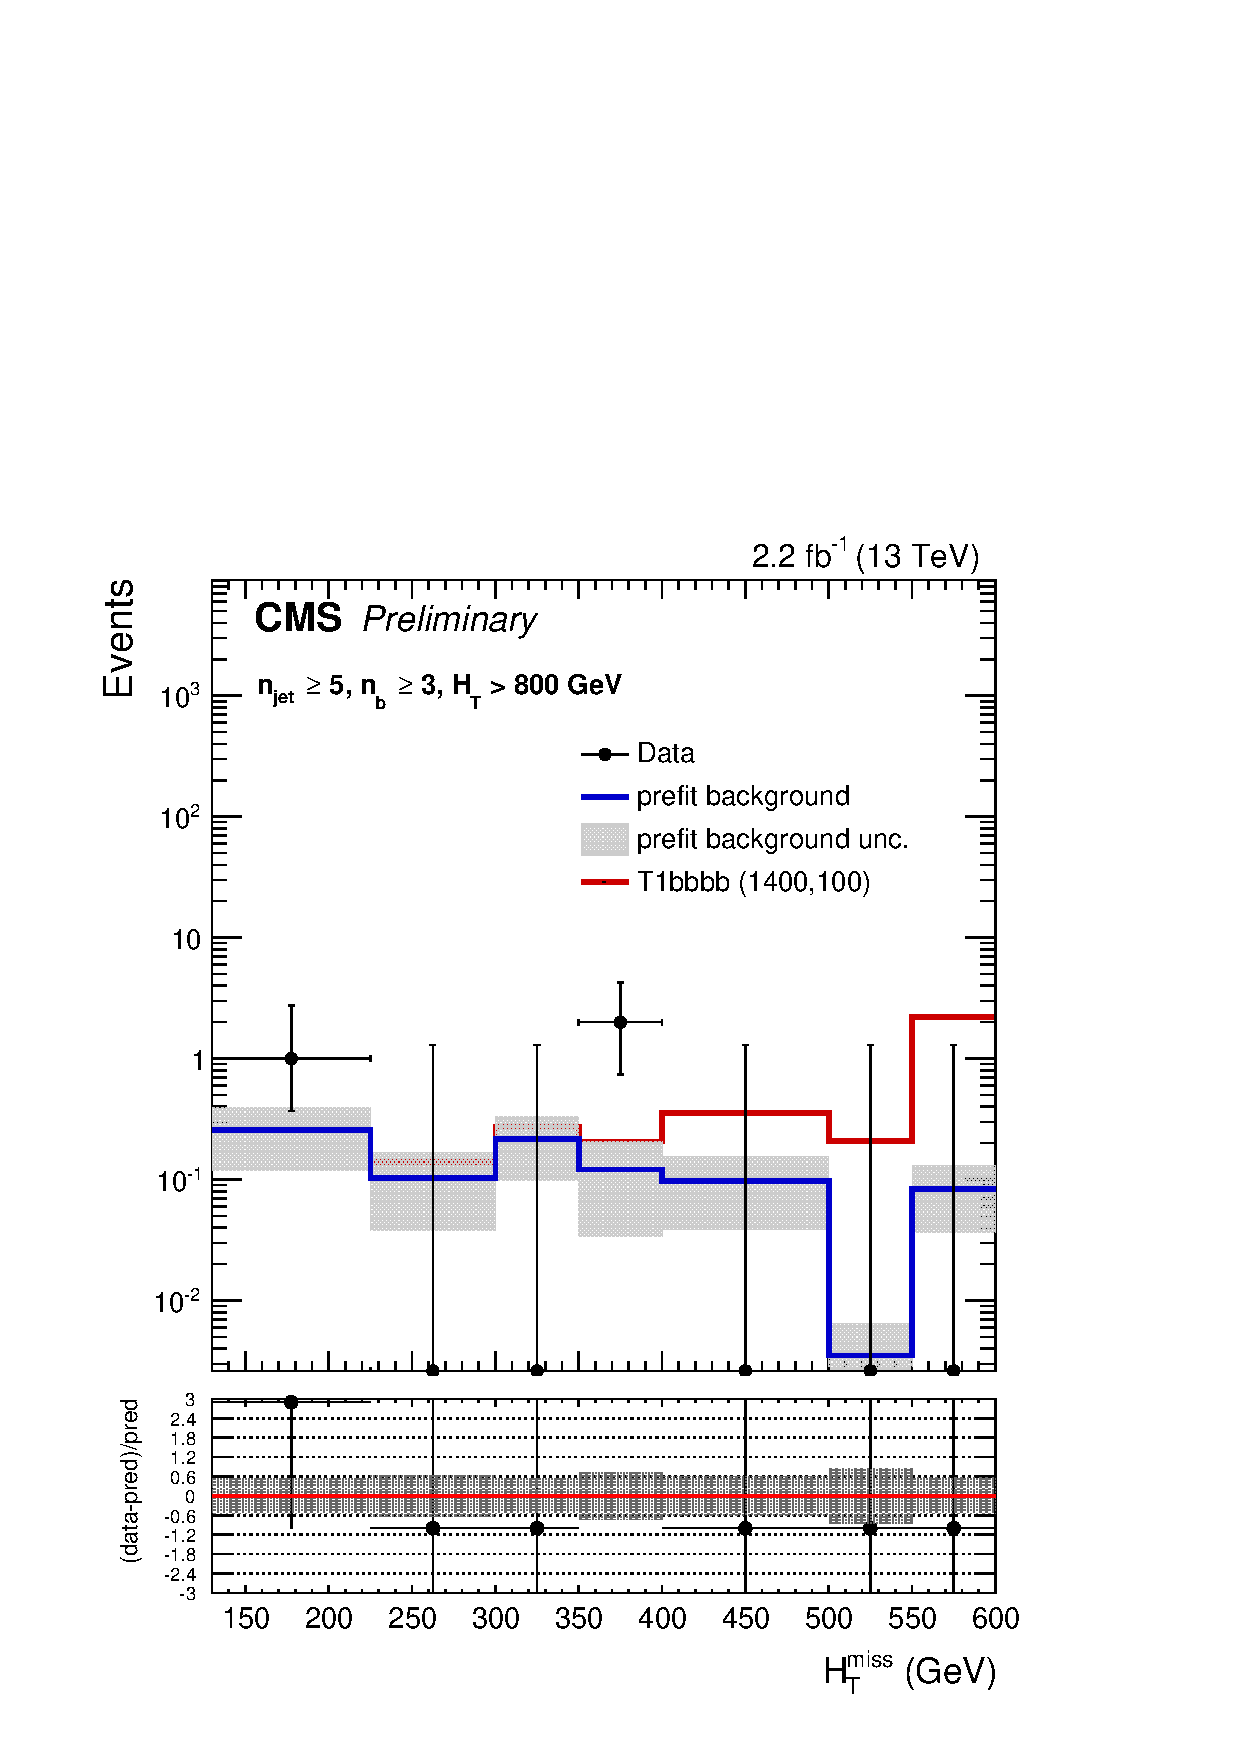
\includegraphics[width=0.5\textwidth]{postFitShape_ge3b_ge5j_800_Inf_prefit} \\
    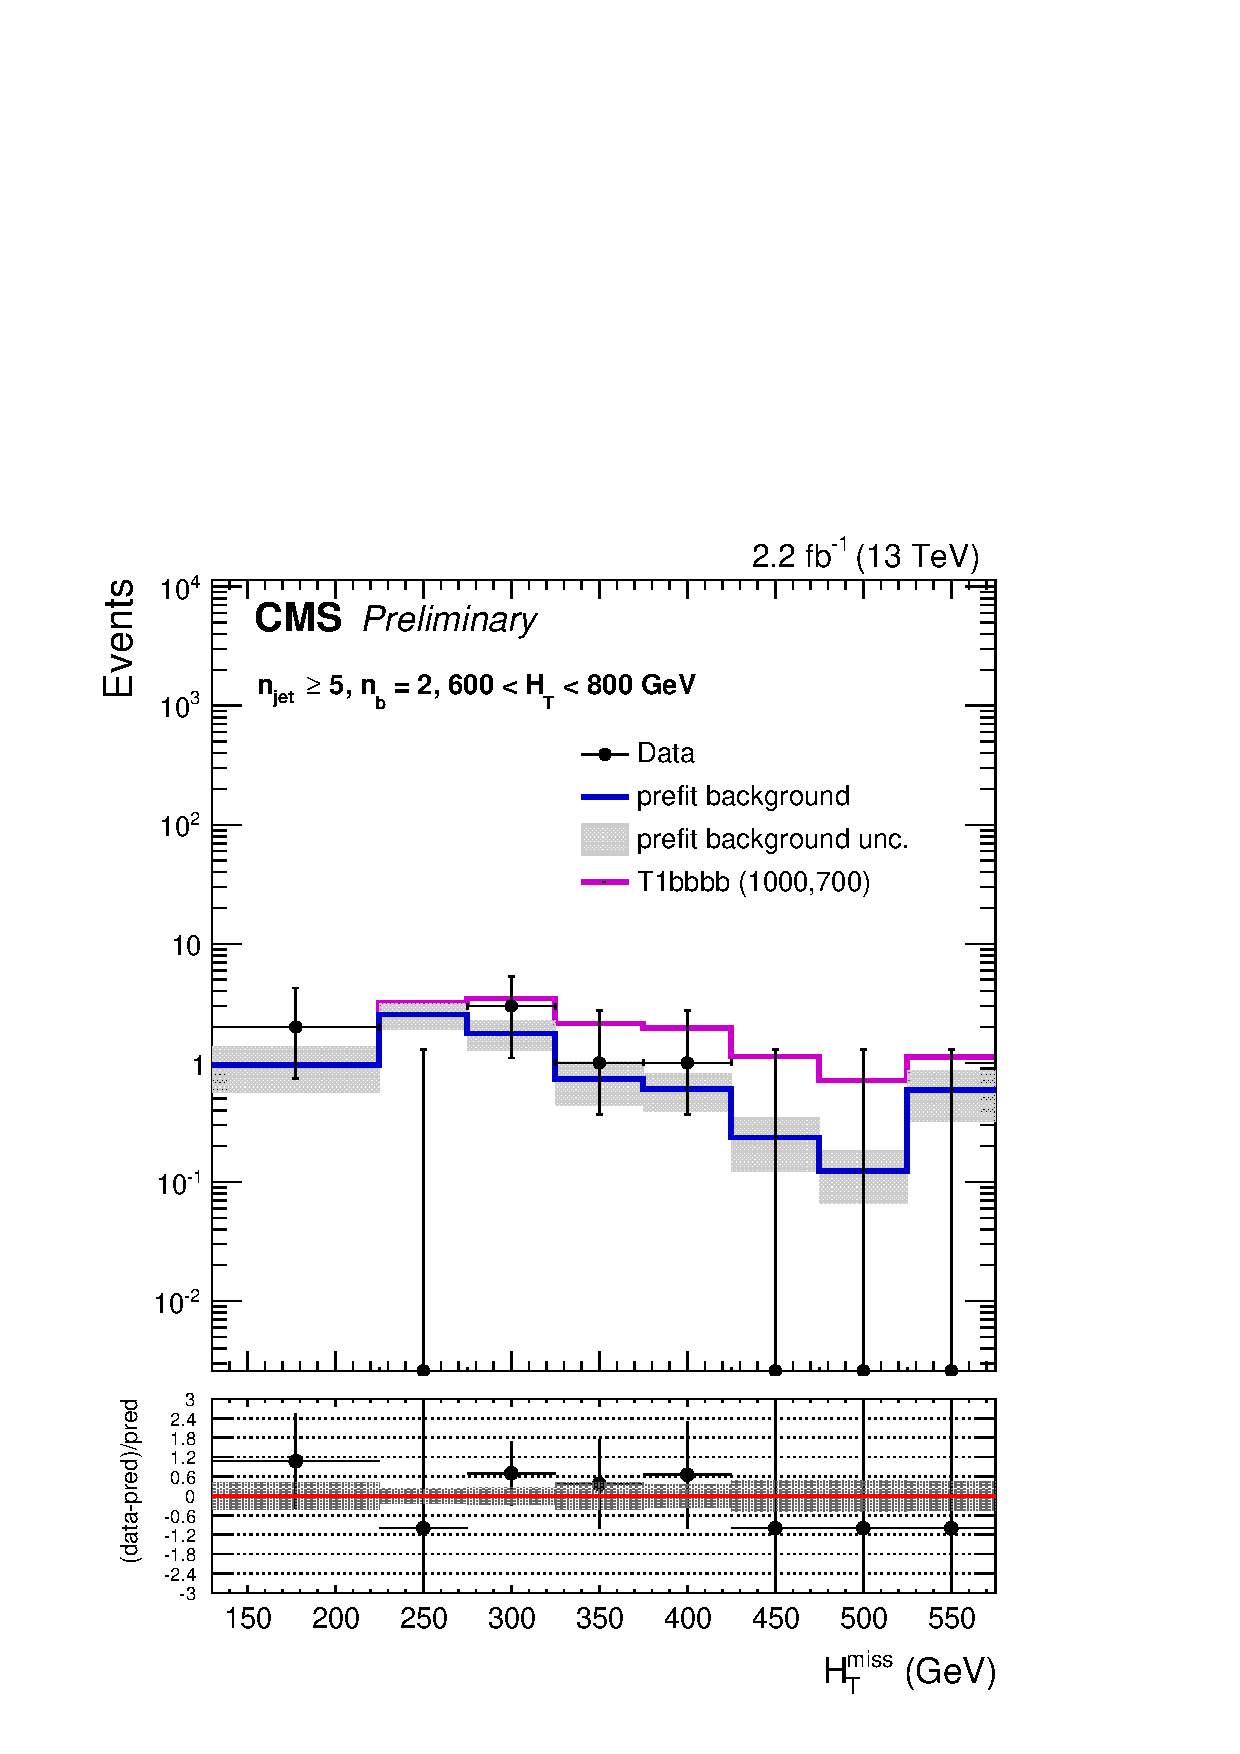
\includegraphics[width=0.5\textwidth]{postFitShape_eq2b_ge5j_600_800_prefit} \\
  \end{center}
  \caption{ The \mht distribution observed in data and the expected
    distribution for the sum of all SM background processes in two
    representative event categories at high \scalht. The expected
    distribution for an example benchmark model with a large (small)
    mass splitting between the gluino and LSP is also shown in the
    left (right) figure. \label{fig:mht-templates} }
\end{figure*}
  
\begin{figure*}[thp!]
  \begin{center}
    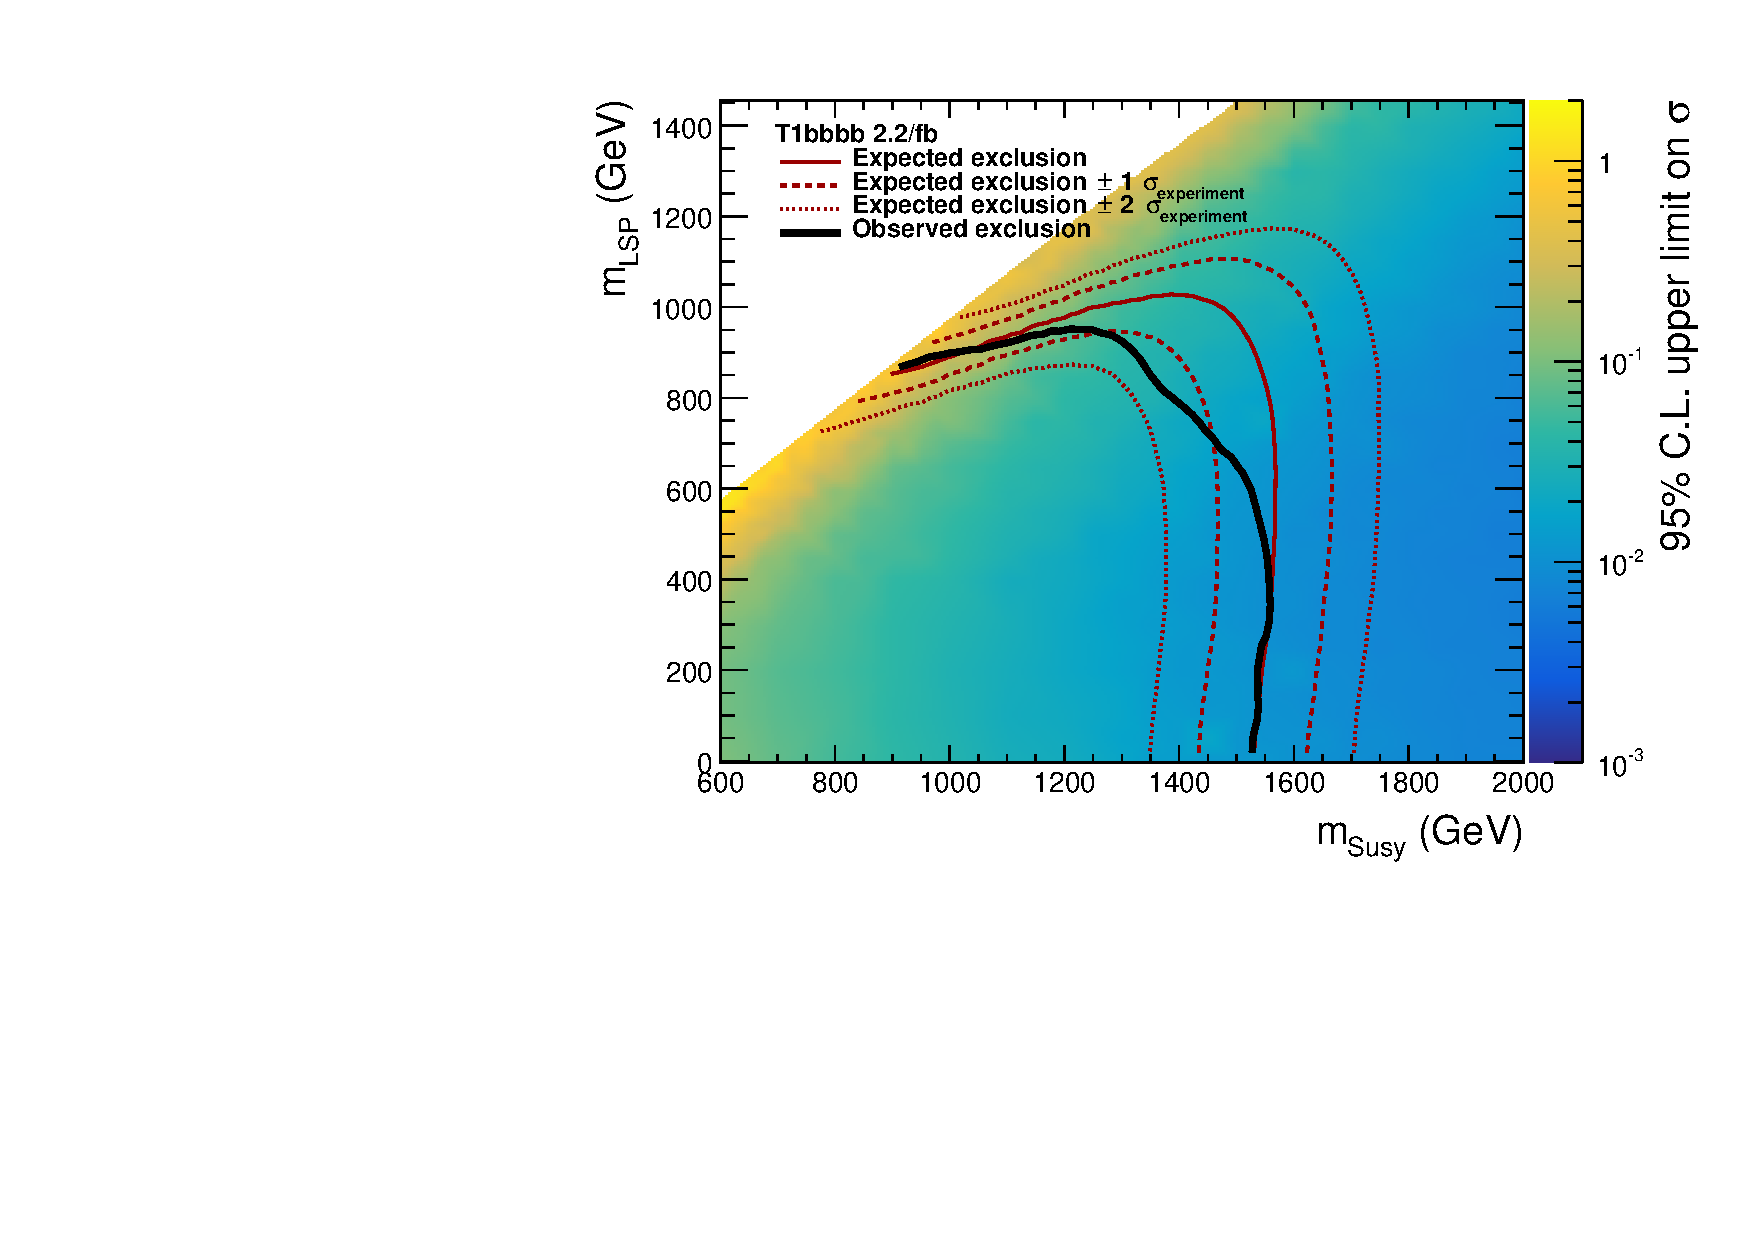
\includegraphics[width=0.49\textwidth]{t1bbbbRA1XSEC.pdf} \,
    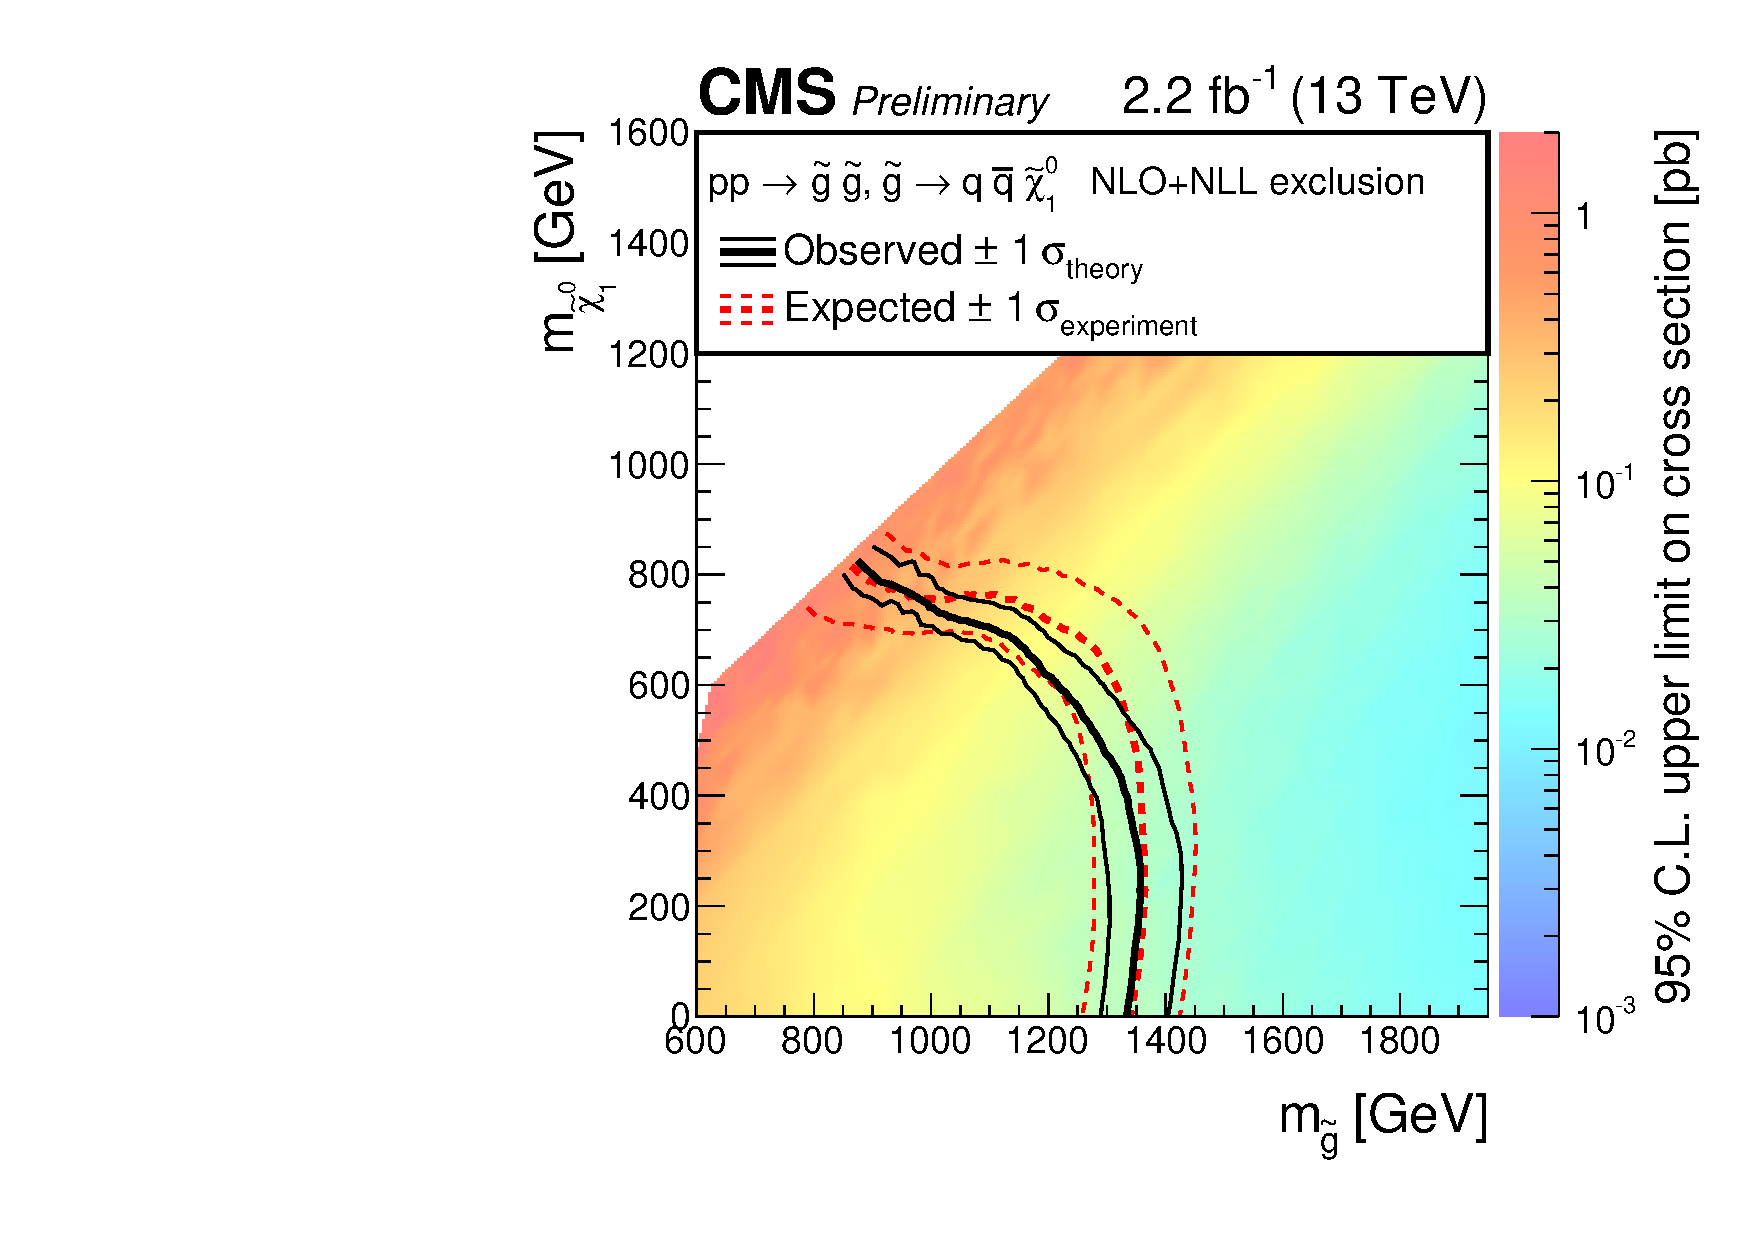
\includegraphics[width=0.49\textwidth]{t1qqqqRA1XSEC.pdf} \\
    \caption{Observed upper limit in cross section at 95\% CL
      (indicated by the colour scale) for simplified models that
      assume the pair production of gluinos, as a function of the
      gluino and $\chiz_{1}$ masses for gluino three-body decays to
      $b\bar{b}\chiz_{1}$ (left) and $q\bar{q}\chiz_{1}$ (right). The
      black solid thick (thin) line indicates the observed mass
      exclusion region assuming the nominal (${\pm}1 \sigma$ theory
      uncertainty) production cross section. The red dashed thick
      (thin) line indicates the median (${\pm}1 \sigma$ experimental
      uncertainty) expected exclusion.
      \label{fig:limits-sms} }
  \end{center}
\end{figure*}

Figure~\ref{fig:limits-sms} shows the observed upper limit on the
production cross section at 95\% confidence level (CL) as a function
of the gluino and LSP masses for a range of simplified models assuming
pair production of gluinos. The observed excluded regions are
determined for gluino pair production assuming decoupled squarks. Also
shown are the observed excluded regions when varying the production
cross section by its theoretical uncertainty, and the expected
excluded region with the ${\pm}1$ standard-deviation ($\sigma$)
variations. The search places stringent limits in the mass parameter
space, with observed exclusions in gluino and LSP masses as high as
$\sim$1550\gev and $\sim$950\gev, respectively.

%%__________________________________________________________________||

\section{Summary}
\label{sec:summary}

An inclusive search for new-physics phenomena is reported, based on
data from pp collisions at $\sqrt{s} = 13\TeV$. The data are recorded
with the CMS detector and correspond to an integrated luminosity of
$2.3 \pm 0.1 \fbinv$. The final states analysed contain one or more
jets with large transverse momenta (\Pt) and a significant imbalance
in transverse momentum, as expected from the production of massive
coloured SUSY particles, each decaying to SM particles and the lightest
stable, weakly-interacting SUSY particle.

Signal candidate events are categorised according to the number of
reconstructed jets, the number of jets identified as originating from
b quarks, and the scalar (\scalht) and the magnitude of the vector
(\HTmiss) sums of the transverse momenta of jets.  The search employs
the use of several kinematic variables, including \alphat and \bdphi,
to suppress the background from QCD multijet production to the percent
level with respect to other nonmultijet SM backgrounds, which are
dominated by vector boson and top quark pair production. The \alphat
variable is also employed in the trigger logic that is used to record
the candidate signal events, which allows the use of low thresholds
for the momentum sums $\scalht > 200\GeV$ and $\HTmiss \gtrsim
130\GeV$. These low thresholds, in addition to the inclusion of final
states containing a single jet, maximise the experimental acceptance
to new-physics processes, such as low-mass squark signatures, nearly
mass-degenerate SUSY models, and other new-physics phenomena, such as
DM models that postulate the direct production of stable, weakly
interacting, massive particles in pp collisions.

The sums of the standard model backgrounds are estimated from a
simultaneous binned likelihood fit to the observed yields for samples
of events categorised according to \njet, \nb, \scalht, and \HTmiss in
the signal region and in \mj, \mmj, and \gj control regions. The
observed yields in the signal are found to be in agreement with the
expected contributions from standard model processes.  The search
result is interpreted in the mass parameter space of fourteen
simplified SUSY models that assume the pair production of
gluinos or squarks and a range of decay modes. The models cover
scenarios that involve the gluino-mediated or direct production or
light- or heavy-flavour squarks, spectra with intermediate SUSY particle
states and nonunity branching fractions, ``natural'' spectra with
gluinos and on-shell top squarks, and nearly mass-degenerate spectra.

The increase in the centre-of-mass energy of the LHC, from 8 to
13\TeV, provides a significant gain in sensitivity to heavy particle
states such as gluinos. In the case of pair-produced gluinos, each
decaying via an off-shell b squark to the b quark and the LSP, models
with masses up to $\sim$1.6 and $\sim$1.0\TeV are excluded for,
respectively, the gluino and LSP. These limits improve on those
obtained at $\sqrt{s} = 8\TeV$ by, respectively, $\sim$250 and
$\sim$300\GeV. In the case of direct pair production, models with
masses up to $\sim$800 and $\sim$350\GeV are excluded for,
respectively, the b squark and LSP. These mass limits are sensitive to
the assumptions on the squark flavour and the presence of intermediate
states, such as charginos.

Finally, a comprehensive study of nearly mass-degenerate models
involving top squark pair production is performed. The two decay modes
open to the top squark are considered: the loop-induced two-body decay
to the neutralino and one c quark, and the four-body decay to the
neutralino, one b quark, and an off-shell W boson. A third scenario is
considered, when the two modes are simultaneously open, each with a
branching ratio of 50\%. Masses of the top squark and LSP up to,
respectively, 400 and 360\GeV are excluded, depending on the decay
modes considered.

In summary, the analysis provides sensitivity across a large region of
the ``natural'' SUSY parameter space, as characterised by
interpretations with several simplified models. In particular, these
studies improve on existing limits for nearly mass-degenerate models
involving the production of pairs of top squarks.

\clearpage

%%__________________________________________________________________||
% \nocite{*}
\bibliography{auto_generated}

%%__________________________________________________________________||
